
\section{Results}
\label{sec:cases}
% \begin{figure*}[!ht]
% \centering
% 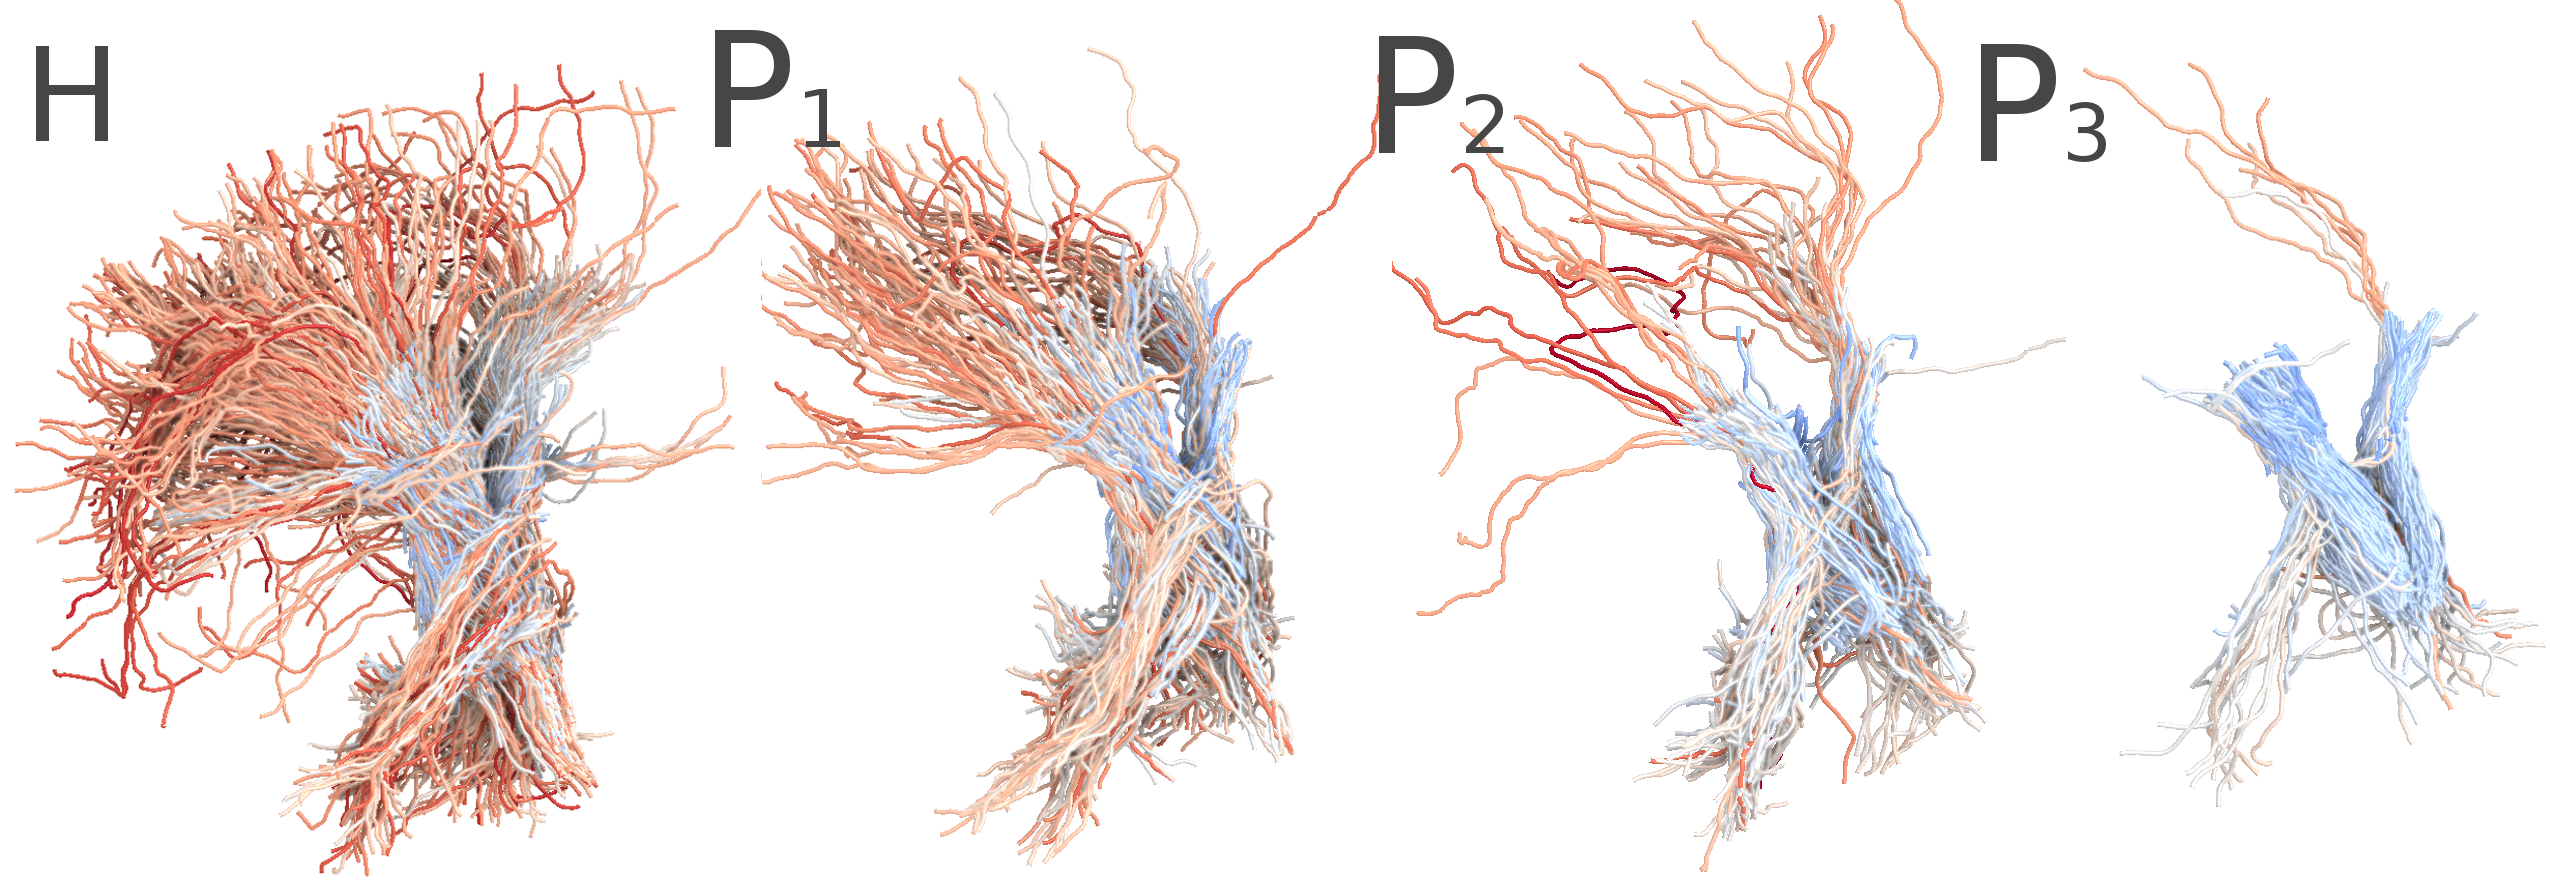
\includegraphics[width=1.0\textwidth]{degeneration.png}
% \caption{The type and severity of fiber loss found among some of the disease group subjects. On the left $(H)$ shows a typical full intact region from a control group subject. $P_1$ through $P_2$ show progressively worse cases of fiber loss. This is a characteristic observed within the disease group, but the severity depicted in $P_2$ and $P_3$ were quite rare, and some apparent loss was observed within control group subjects as well.}
% \label{fig:loss}
% \end{figure*}

\noindent % Each of 
Our studies are based on DTI images and %reconstructed 
derived fiber tracts of Parkinson's and Control groups obtained from the 
%research 
database of PPMI~\cite{marek2011parkinson}.  

% \begin{figure}[!t]
% \centering
% 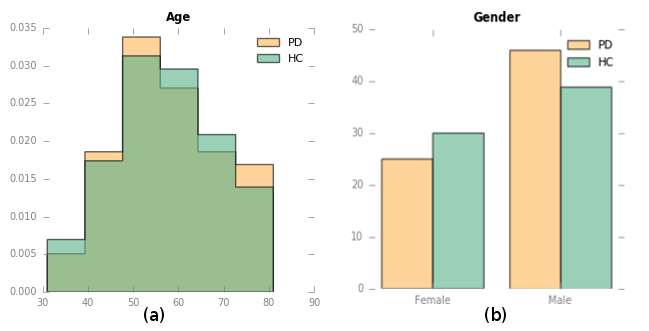
\includegraphics[width=1\textwidth]{images/Demographic.png}
% \caption{Demographics of the dataset. The age distribution (a). The two sets of data have similar age distributions. The gender distribution (b). In both disease group and HC, the amount of male data is more than that of female.("The incidence of Parkinson’s disease is low before
% the age of 50 years, but it increases rapidly with age,peaking in most studies at around 80 years, probably
% because of underdiagnosis with increasing age" -- copy from \cite{ASCHERIO20161257})}
% \label{fig:demographic}
% \end{figure}



\subsection{Data Acquisition and Processing}

\noindent MRI parameters, such as gradient direction, b-value, and voxel resolution, have a crucial impact on the scalar measurements that are used for clinical study. To prevent errors, the MRI images provided by PPMI, were collected based on standardized and strict acquisition protocols developed by the steering committee on 3T Siemens scanners.

Each subject includes DTI and T1-weighted images. For each DTI image, a 2D echo-planar DTI sequence was acquired with the following parameters: TR = \SI{900}{ms}, TE = \SI{88}{ms}, Image matrix $= 116\times116\times72$ and voxel resolution $ = 1.98\times1.98\times2$\SI{}{mm^3}, 64 gradient volumes (b = \SI{1,000}{s/mm^2}), and one non-gradient volume (b = \SI{0}{s/mm^2}). The acquisition parameters for T1-weighted images are as follows: TR = \SI{2,300}{ms}, TE = \SI{2.98}{ms}, Image matrix $= 160\times240\times256$ and voxel resolution = $ 1\times1\times1$\SI{}{mm^3}.

Both the DTI and T1-weighted images require preprocessing, since a variety of issues affect fiber tracking results, such as intensity loss, blurring, gradient distortion, and inhomogeneities in the applied magnetic field. Correction is required to accurately estimate fiber orientation and achieve alignment from DTI to T1-weighted images, which would affect MRI coregistration (intra-subject registration) and cause great deviation in the extracted fibers from Regions of Interest (ROI).

% All DTI and T1-weighted images were converted from the Digital Image and Communications in Medicine (DICOM) format to Neuroimaging Informatics Technology Initiative (NIFTI) format. 

For our study, DTI images were processed using MRtrix3~\cite{mrtrix3}. We first denoised each DTI, and then performed Echo-planar Image/fieldmap correction, eddy current correction, and head motion correction; finally, we performed B1 field inhomogeneity correction for the DWI volume series. The preprocessing procedures for T1-weighted images are based on FreeSurfer~\cite{freesurfer}, including motion and non-uniformity correction. T1-weighted image volumes were registered to the DWI images using FSL~\cite{fsl}. % 5.0.10~\cite{fsl}.

Brain fiber tractography was performed using a state of the art framework~\cite{SMITH20121924}, which can reconstruct neuronal axons and retain biological accuracy. This framework was also used to generate the tract-based, and tensor-based features. 

\subsection{Disease Background}

\noindent PD is a neurodegenerative disorder characterized by loss of dopamine neurons in the substantia nigra (SN) brain region~\cite{prakash2012asymmetrical}. The dopaminergic function of the nigrostriatal pathway reduces with the depletion of these neurons, as well as the neural fibers that link the SN to other subcortical regions, such as putamen and caudate \cite{zhang2015diffusion}. Each region in the mid brain is affected based on the anatomical correlation with SN and the severity of the region reflected by the functional relationship with SN. %\cite{zeighami2015network}. 
It is recognized to be a brain-wide neurodegenerative process that spreads up from brainstem into the cortex, as originally suggested by Braak.etc~\cite{yau2018network}. %Significant effects were also observed in the whole Parkinson's disease brain with spatial distribution of quantitative susceptibility mapping (QSM) \cite{atkinson2017diffusion}. 
PD also increases rapidly with age, with low incidence before 50, and most cases found around 80~\cite{ASCHERIO20161257}. Once the fibers are detected by tractography, it is useful to assess the diagnosis with the brain fiber pathways. 

% \begin{figure*}[t]
% \centering
% 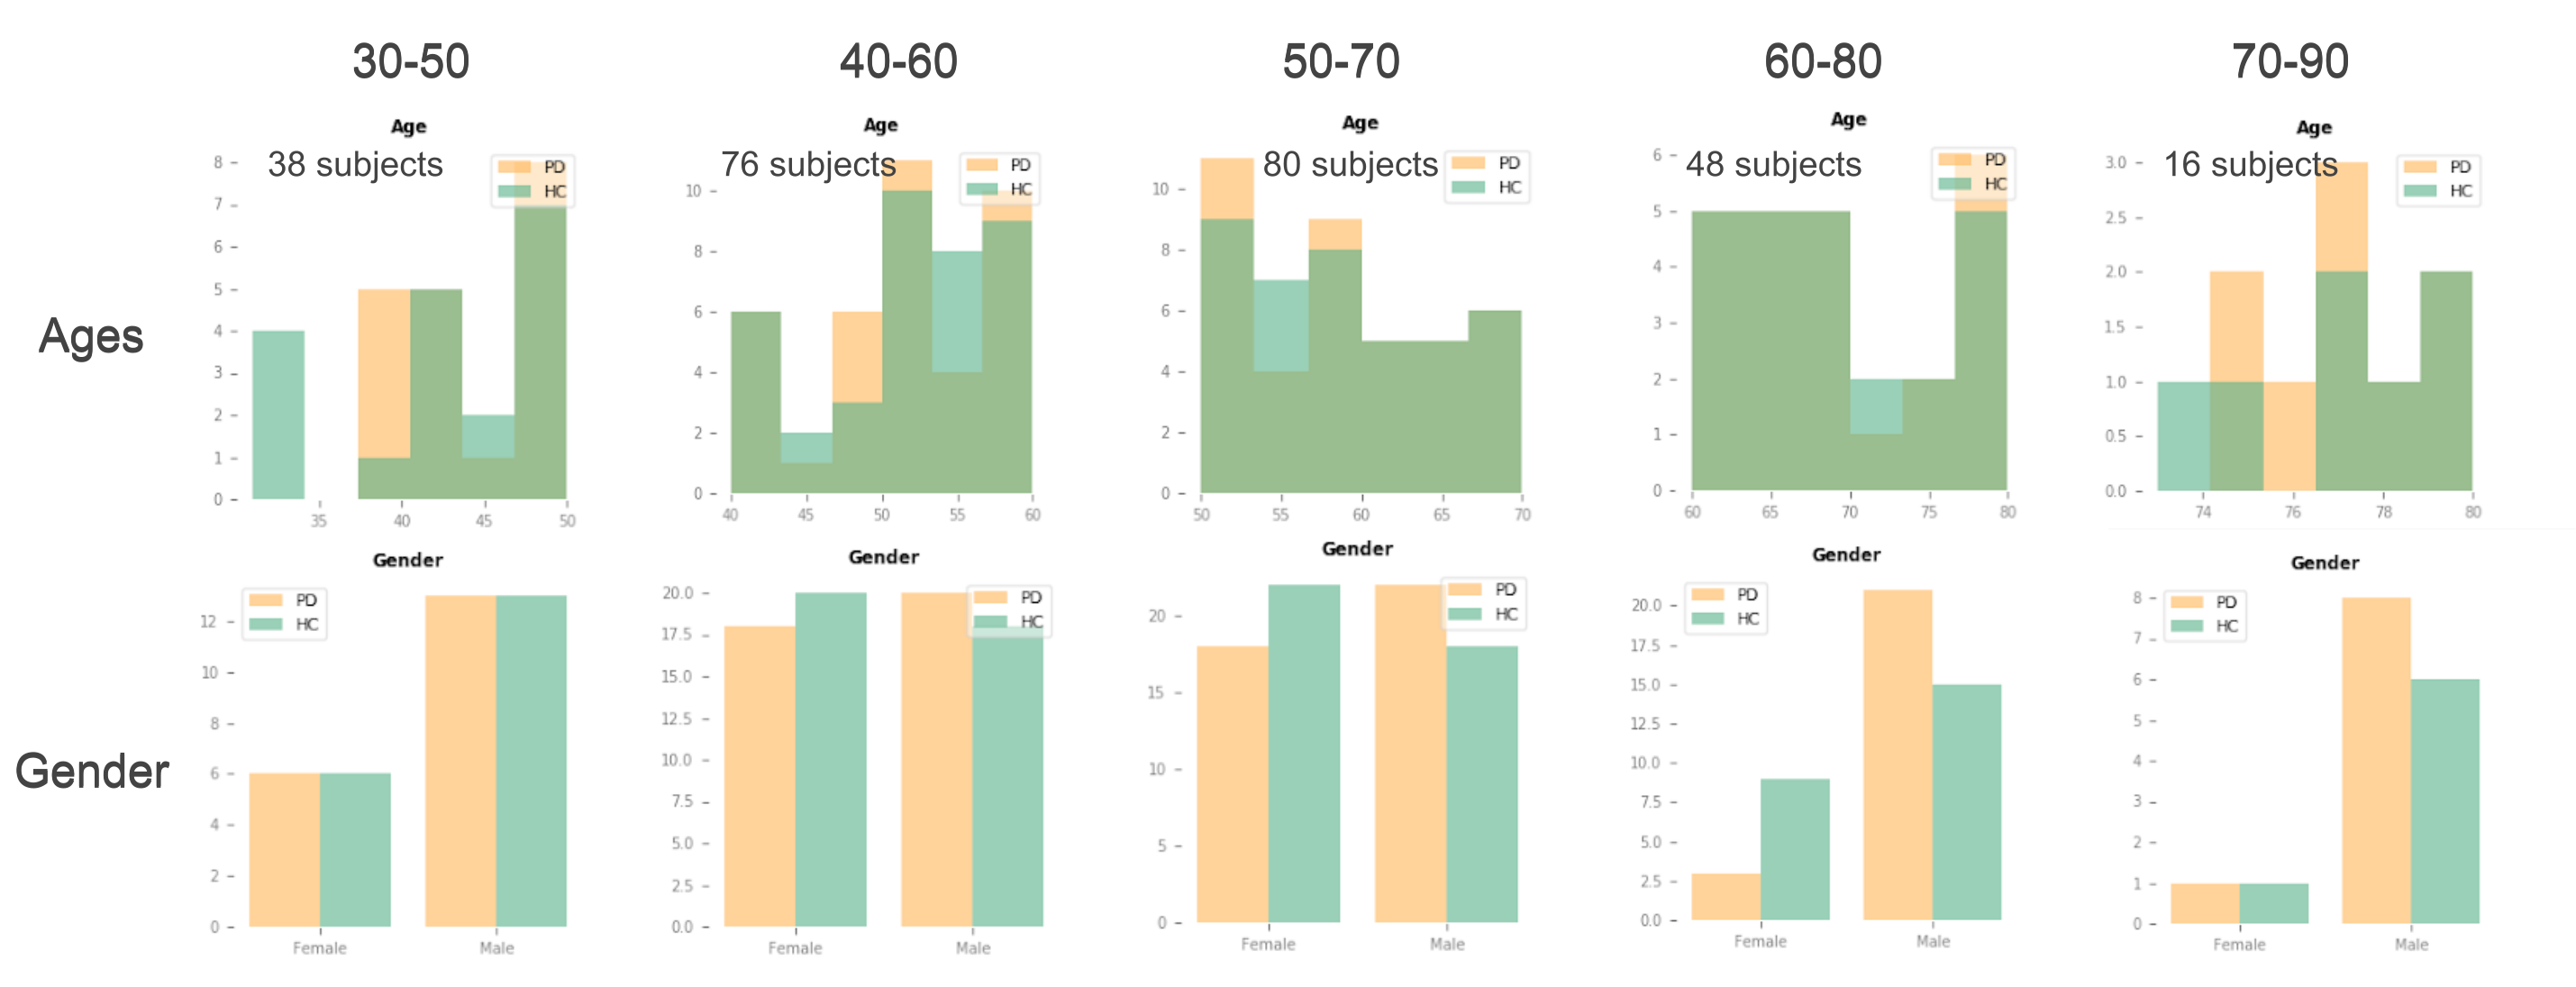
\includegraphics[width=0.85\textwidth]{images/groupsDemographics.png}
% \caption{Age and gender distributions of 5 subgroups, which have been divided by ages with 20 as the step size. The first row shows the age distributions of each subgroup, while the second row shows gender distributions. 
% In the age distribution histograms, the overlap part of the HC and disease group is drawn in light green.}
% \label{fig:groupDemographics}
% \end{figure*}



% \begin{figure*}[t]
% \centering
% 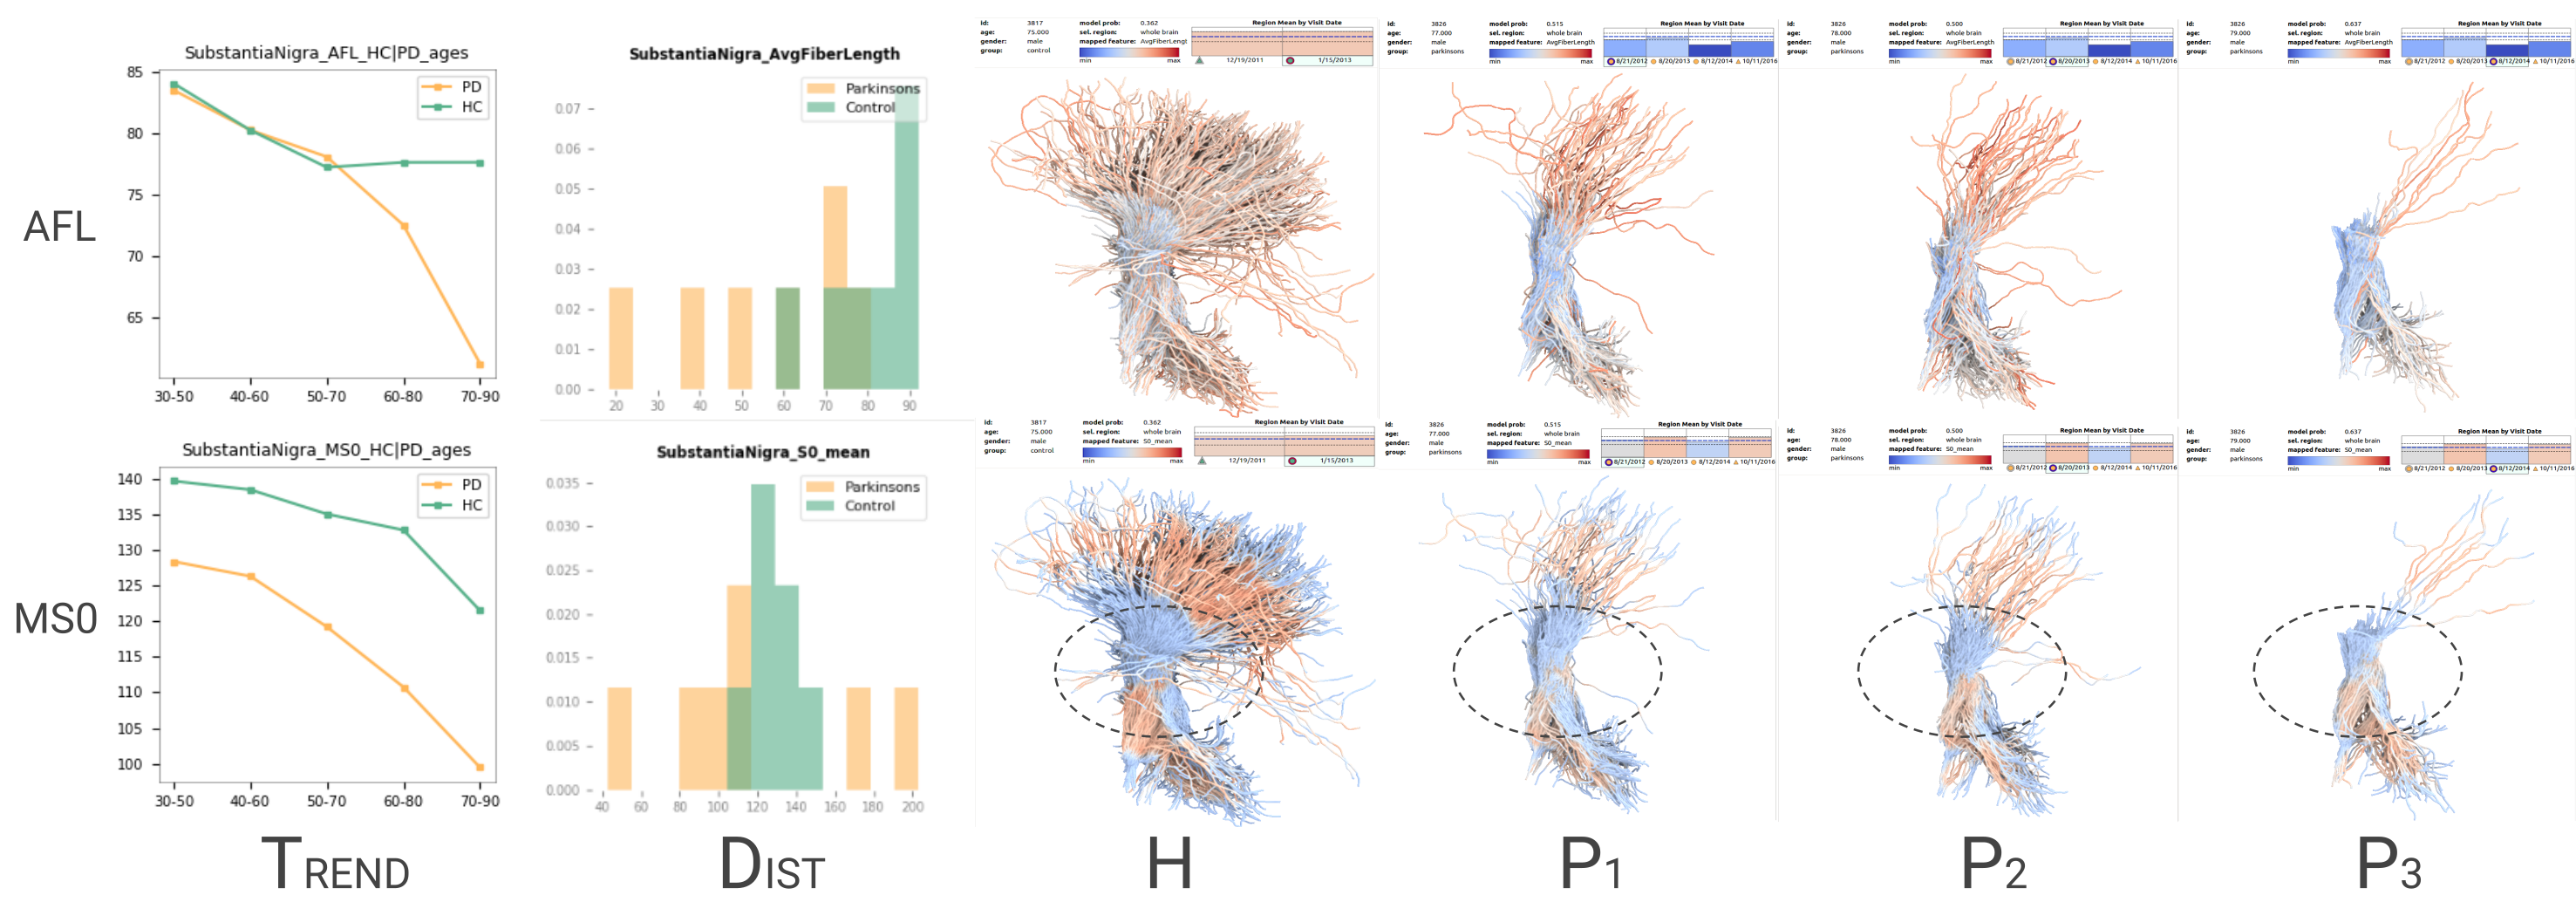
\includegraphics[width=0.85\textwidth]{images/SNcase_v3.png}
% \caption{ PD effects in nigrostriatal fibers and tensor features within the elderly group. The $Trend$ column shows the feature changes in different ages. The $Trend$ column shows the views for comparing the groups' distributions of the selected feature. $H$ column shows the nigrostriatal fibers of a subject from the HC, while $P1$ to $P3$ show the nigrostriatal fibers of a subject in different years. The two rows show two different feature performance on PD. $AFL$ is short for average fiber length, and $MS0$ indicates mean value of raw T2 signal with no diffusion weighting.}
% \label{fig:SNcase}
% \end{figure*}
%\textbf{D}\text{\small{IST}}

% \subsection{Case Study 1: Exploration of Parkinson's Disease with the Nigrostriatal ROI}

\subsection{Study 1: Exploration of PD with the Nigrostriatal ROI} %(a

\begin{figure*}[t]
\centering
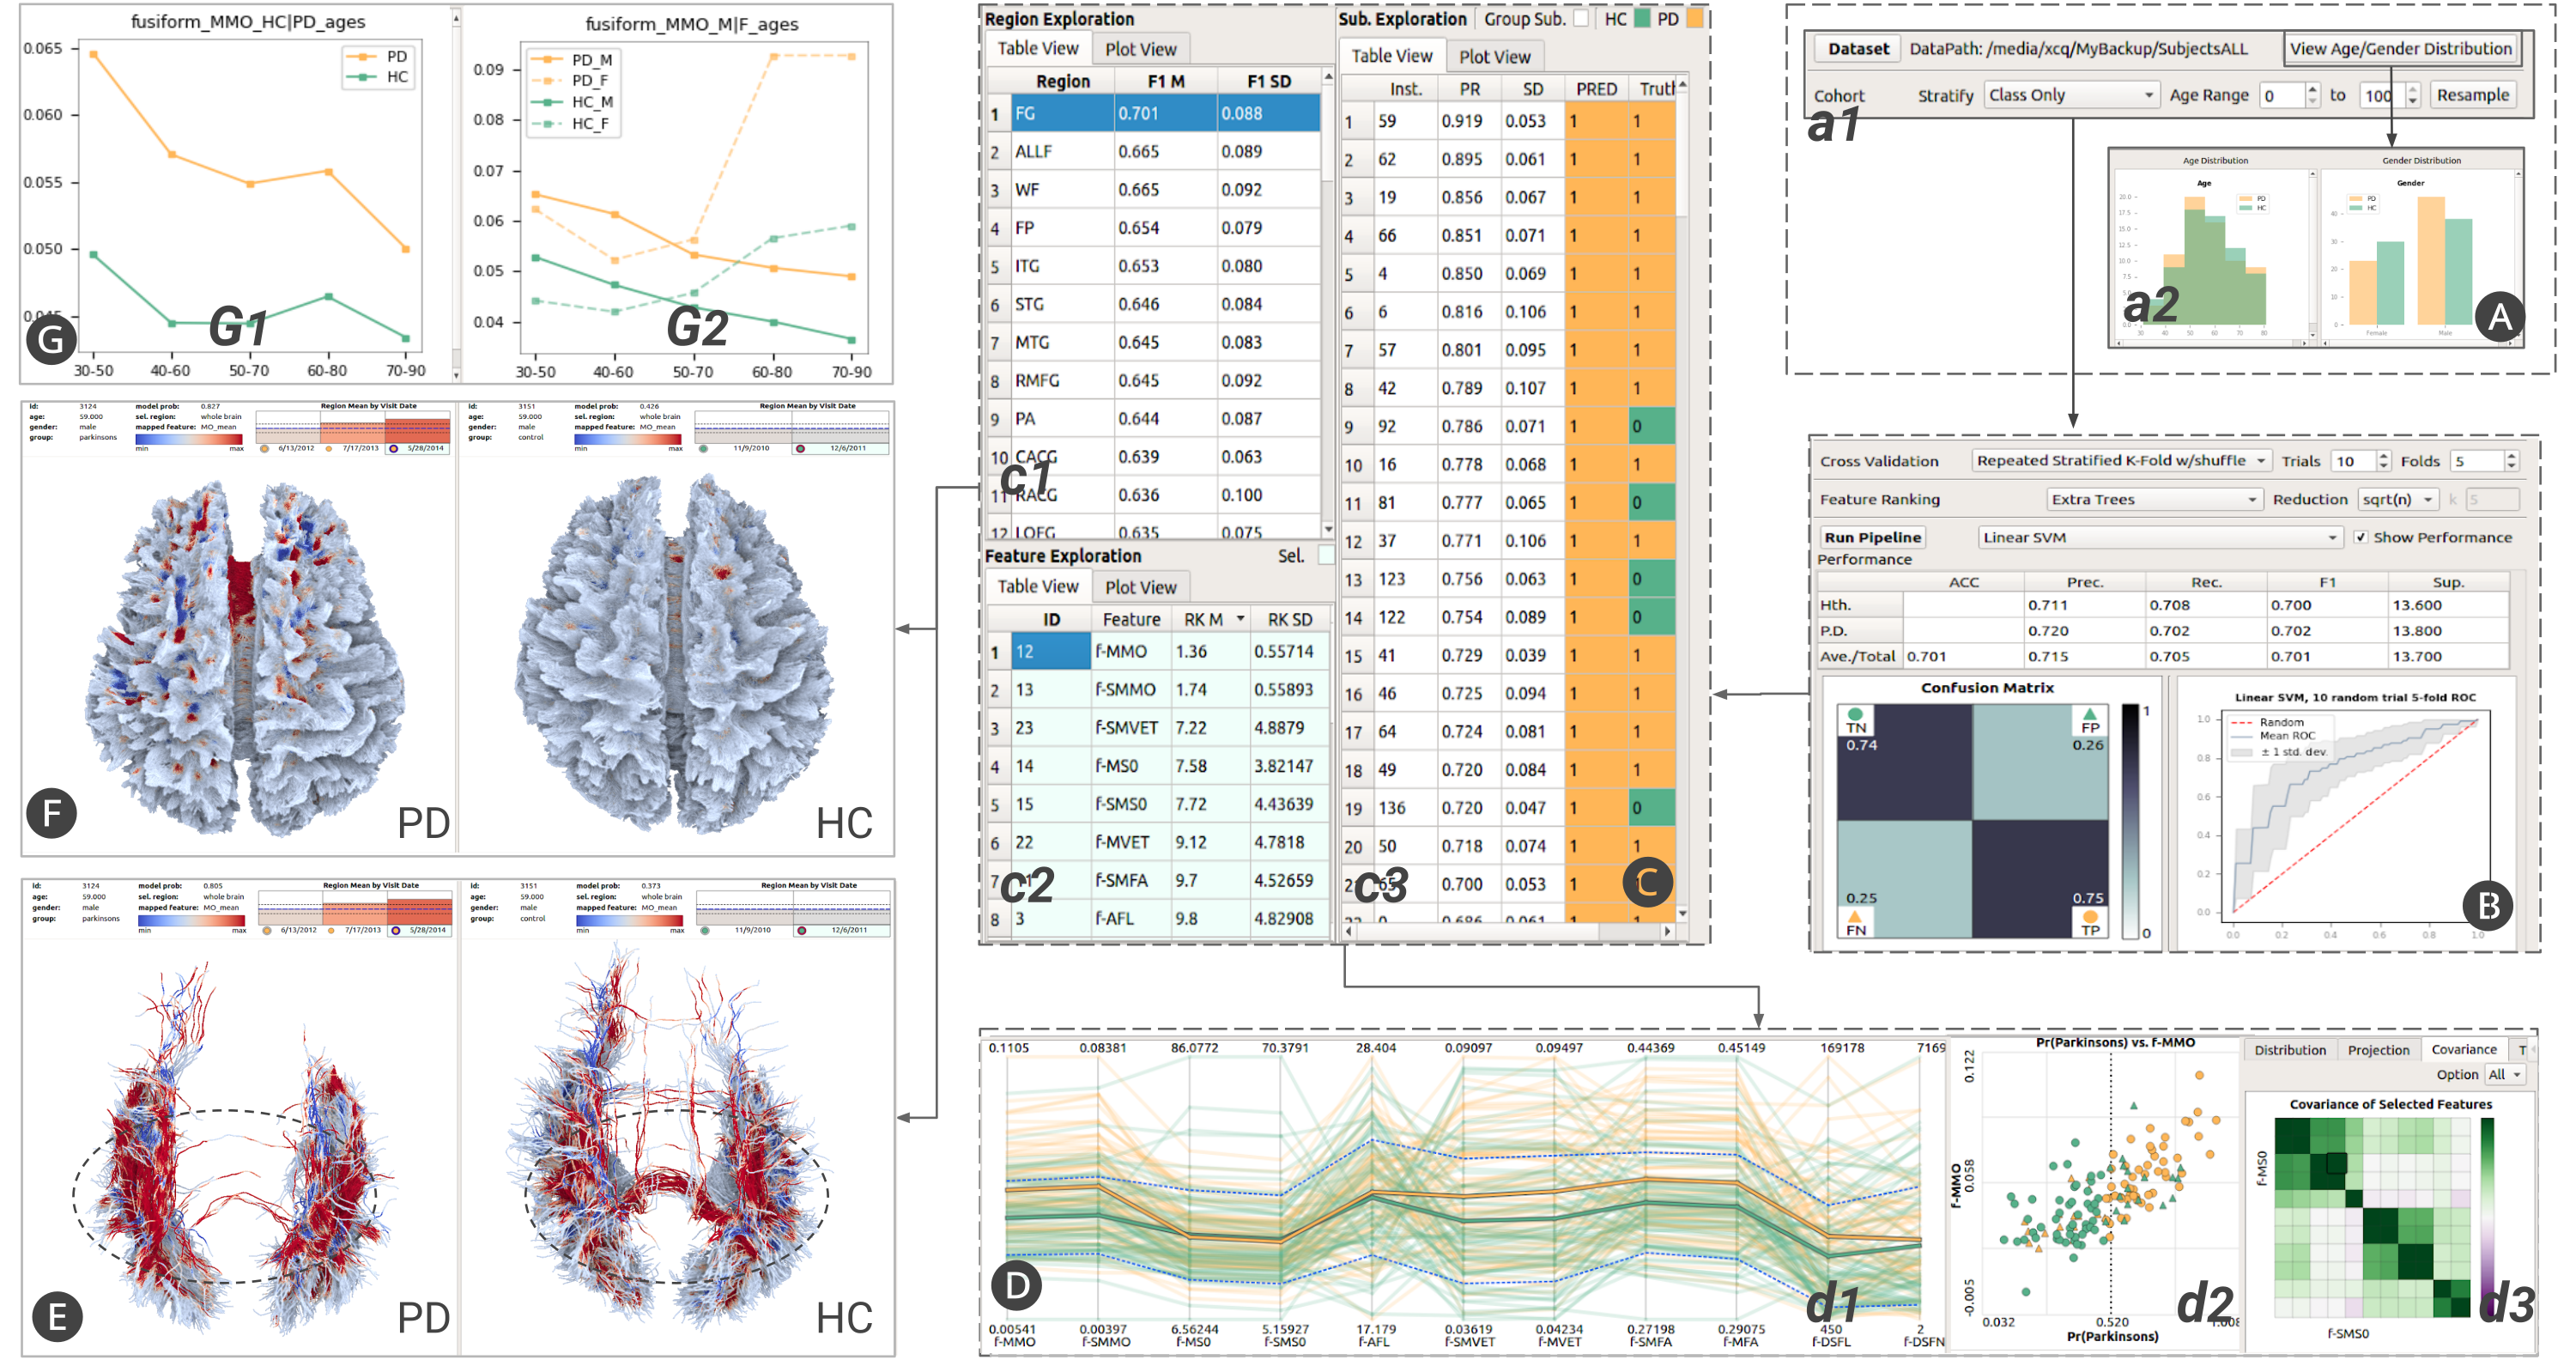
\includegraphics[width=0.95\textwidth]{images/fusiformSteps_v5.png}
\caption{ Data selection module \glf{A}, entering an age range from \textbf{\textit{a1}} and displaying the distribution in \textbf{\textit{a2}}. ML module \glf{B}. users can run ML algorithm with input parameters. Prediction results module \glf{C}. Brain regions \textbf{\textit{c1}}, features \textbf{\textit{c2}}, and subjects \textbf{\textit{c3}} were sorted in the table. Information visualization module \glf{D}. parallel coordinate \textbf{\textit{d1}}, partial dependence plot \textbf{\textit{d2}}, and covariance matrix view \textbf{\textit{d3}} were used to show the distributions and relations of the features and subjects. 3D rendering module \glf{E} and \glf{F}. Brain fibers were rendered in the juxta-positioned 3D rendering views for visual comparison with timeline views of the selected subjects. Group trends plotting module \glf{G} ( trends with age \textbf{\textit{G1}} and trends with gender \textbf{\textit{G2}}).}
\label{fig:fusformSteps}
\end{figure*}

\noindent Based on the disease background,
% that PD is histopathologically characterized by the loss of dopamine neurons in the substantia nigra pars compacta, 
we decide to explore fiber bundles with streamlines starting from the SN region; our focus is on trends with age, and spatial feature patterns from older subgroups (where significant symptoms have been reported). Age based exploration is achieved through a 2 stage process.  
%, an important region to study as found in the medical literature on Parkinson's and other neurodegenerative diseases. 
% In this case study, we are interested in the following tasks
% : 1) Compare group level nigrostriatal feature trends and distributions. 2) Inspect and compare the patterns and variations of dis-aggregated features in the physical space, and inspect the fiber structure on a per-brain level to seek an intuitive understanding of observed physiological differences with PD progression. %3) Decompose and analyze trends by age and gender.

%1) Analyze nigrostriatalfeature patterns. Compare the distribution of the features differ fromPD subjects and HC subjects. 2) Identify the physical characteristics ofthe nigrostriatal fibers. Understand the physical structure differences innigrostriatal fibers between HC and PD subjects and have an intuitiveunderstanding of the nigrostriatal fibers changes in PD progress.  3)Age-related nigrostriatal fiber analysis. Get an overview of the featurechanges and physical structure changes in different age groups 
First, from the entire sample, we investigate average trends by age (split by class and gender as in Fig.~\ref{fig:infovis} \glf{B}). In this case, we look at average fiber length in the SN region (s-AFL) as shown in Fig.~\ref{fig:SNSteps} \glf{H}. We see a decreasing trend for elderly male subjects with PD. As we investigate the trend, we begin selecting individual subjects to highlight in the plot (using the mouse). This helps us relates the trend with subject level behaviours. We can then investigate outliers, and make comparisons between subjects, and across the linked views. We note a high level of variability in some subject's time-point evolution, which gives us a sense of the uncertainty due to fluctuation.

Next, we re-sample the dataset into groups of only elderly subjects, as shown in Fig.~\ref{fig:SNSteps} \glf{A} \textbf{\textit{a1}}. One issue that we contend with, is that we have limited data in this age group, including a significant lack of elderly female subjects. These issues are assessed by viewing the distributions in age and gender as shown in Fig.\ref{fig:SNSteps} \glf{A} \textbf{\textit{a2}}. This helps to understand the limitations of the data, and uncertainty implications before proceeding in the exploration. While our system supports re-sampling to balance the age and gender distributions, (both within, and across classes) this would limit our data to a very small sample when combined with the restriction on age, and would disallow detailed exploration of the discarded subjects. In this case, we selected subjects over 65 years of age. The ML pipeline is then executed using a support vector machine. The average accuracy for the SN region (over all CV trials) is 76.1\%, and average $F_1$ is 0.760 (Fig.~\ref{fig:SNSteps} \glf{B}). 

% The user can then pragmatically explore the sorted features, sorted brain regions, and sorted subjects that based on the rankings and predictions in Fig.~\ref{fig:SNSteps} \glf{C}. In this case, the prediction accuracy reaches 77.5\% and the standard deviation reaches 0.100 (\textbf{\textit{c1}}). 

The top $7$ ranked SN features were average fiber length (AFL), mode of the anisotropy (MO), fiber number (FN), and raw T2 signal with no diffusion weighting (S0), each for the entire ROI and the inner-connect fibers separately (\textbf{\textit{c1}}). After selecting AFL, we look at its distribution between groups and find a notable overall difference; the HC group tends to have higher values (Fig.~\ref{fig:SNSteps} \glf{D}). The parallel coordinates view (\textbf{\textit{d1}}) shows group and individual trends in the top $7$ features'. Several features have PD group averages (thick orange line) beyond one standard deviation of the HC group (thick green line surrounded by blue dotted lines).

Plotting AFL vs Pr(PD) gives insight into the relationship between AFL and the trained classifier (Fig.~\ref{fig:SNSteps} \glf{D} \textbf{\textit{d2}}). A linearly decreasing trend suggests that the trained model is trivially exploiting a correlation between PD labels and AFL in the data for this group. Subjects are then picked out from the exploration module based on strength of prediction and true class (\textbf{\textit{c3}}). They are then compared in the physical space and in the linked information visualization views, where they are highlighted. We first compare the fibers colored by AFL (\glf{E}), and then S0 (\glf{F}). For the selected HC subject, the nigrostriatal fibers are mostly red-orange (indicating higher than average length), while the selected PD subject has more blue fibers (indicating lower than average length). For S0, it seems that values closer to the center of SN are higher in the observed HC subject. The patient time-point module views (\glf{G}) above the fiber views show these subjects have fairly consistent values between different scans, which suggests a level of stability/consistency in imaging, pre-processing and fiber tracking. 

% Selecting the plot types in Fig.~\ref{fig:SNSteps} \glf{H}, the AFL feature distribution with respect to age and gender are shown in \glf{H}, illustrating the impact of those factors on the disease. In the age-related view (\textbf{\textit{I1}}), both the HC group and PD group show a declining trend with age. However, the AFL in the disease group decrease rapidly in elder ages, while in the HC it maintains stable. In the gender-related view (\textbf{\textit{ I2 }}), curves of sexes have been plotted for seeking inner relations between genders. It seems men are more likely to get sick than women. It should be pointed out that the limited subjects, especially the old age subjects, would certainly bring uncertainties in the analysis of the disease. More subjects are needed to get a more confident result \textbf{(Task 3)}.


% \begin{figure}[t]
% \centering
% 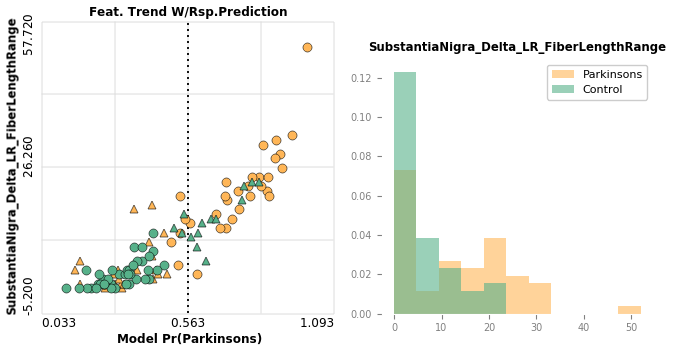
\includegraphics[width=0.9\textwidth]{DSFL.png}
% \caption{Comparing the distributions of the ``Delta-Left-Right Sum of Fiber Lengths" feature (absolute difference in sum of fiber lengths between the left and right hemispheres) between the control group (blue-green) and disease group (orange). Many more subjects from the disease group are within the higher range in the feature value, yet many disease group subjects have small differences from the control group.}
% \label{fig:DSFL}
% \end{figure}

% \begin{figure}[t]
% \centering
% 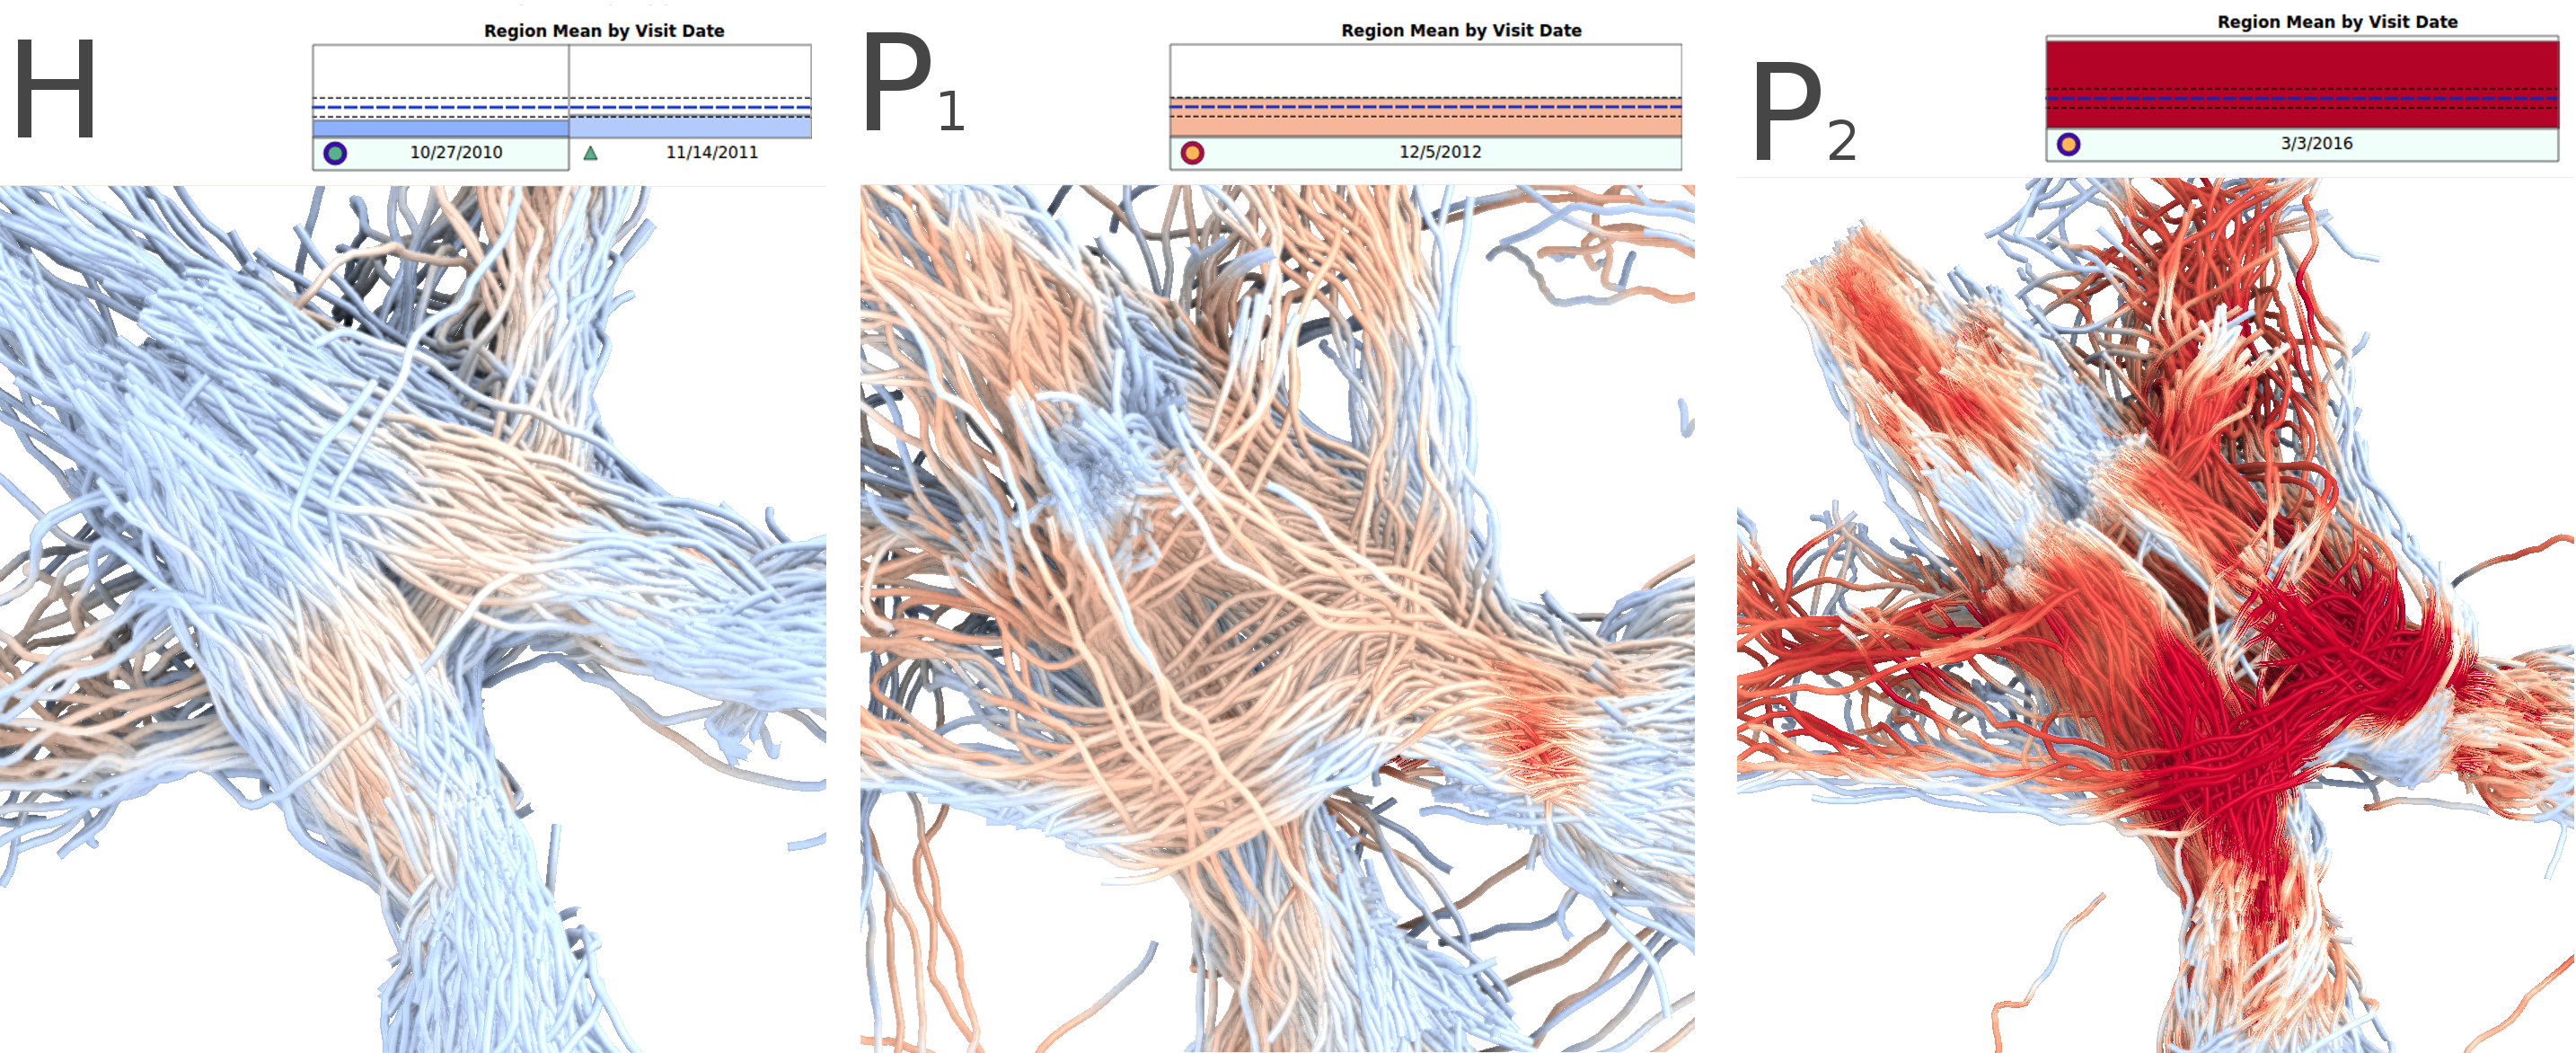
\includegraphics[width=0.9\textwidth]{SSO.png}
% \caption{The substantia nigra region is rendered with the S0 feature (raw T2 signal with no diffusion weighting) mapped using color. In the top $(H)$, the region is for a control subject that has overall lower values, and is without patches. This characteristic seemed more prevalent within the control group, yet many disease group subjects have this characteristic as well. The next two images $(P_1, P_2)$ each show brains fiber tracts from the disease group. In the middle $(P_1)$, patches of high values are observed in areas near the mid-section of the region. This characteristic seemed more prevalent in the disease group, yet is also found in many control group subjects as well. In the bottom ($P_2$), an example of a subject with abnormally high signal values throughout the mid-section and outer sections of the region. This effect seemed more prominent in more disease group subjects, yet was observed in some control group subjects as well.}
% \label{fig:SSO}
% \end{figure}


% \begin{figure}[t]
% \centering
% 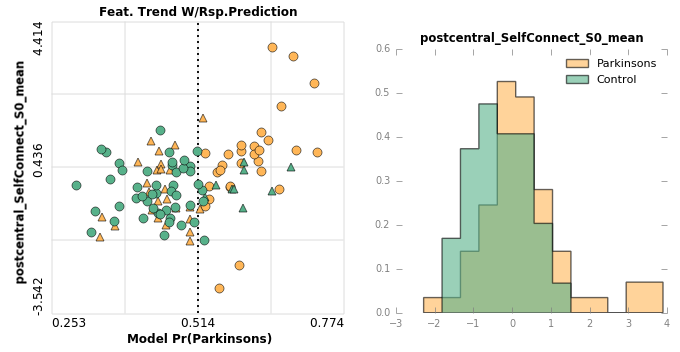
\includegraphics[width=0.9\textwidth]{PMSO.png}
% \caption{Comparing the distributions of the S0 feature (raw T2 signal with no diffusion weighting) between the control group (blue-green) and disease group (orange). The disease group's distribution is centering at a higher value than the control group and there are multiple outliers from the disease group in the high value range.}
% \label{fig:PMSO}
% \end{figure}


% \subsubsection{Analysis and Insights}

Based on the findings from previous works, we expected SN to be a high ranked region. However, with our data, we were only able to find noteworthy differences in older groups. As we seek to isolate smaller ranges of age, we run into problems where we don't have enough examples to make confident inferences. In addition, we find high variation in fiber features between individuals, making clear associations difficult. These problems can be addressed in further work using our system as data collections increase in size, and experts are able to refine the ROIs and feature engineering to better isolate the important differences.   

% Due to the limited data size and the unbalanced data distribution, we initially split the data into 5 subgroups with a step size 20. Fig.~\ref{fig:groupDemographics} shows the demographics of the flatted 5 subgroups with balanced age and gender factors. In general, the prediction accuracy increase from 60\% to 90\% with age growth.

% Fig.~\ref{fig:SNcase} shows parts of our findings within the elderly group, with age from 70 to 90. Significant differences have been discovered that related to the AFL feature, one of the top scoring feature for the nigrostriatal fibers. Generally, as seen in the $Trend$ column, the AFL decreased in both HC and PD subjects at early ages. However, the HC group keeps the AFL steady, while in PD group it has a tendency of rapid decline. From the distribution of fiber length (the $DIST$ column), it is easy to find that the HC group overall has longer nigrostriatal fibers than the PD group. The third column image shows a typical HC group subject which has very complete nigrostriatal fibers, while the right 3 images show progressively worse cases of nigrostriatal fiber loss of a PD subject in different time steps. The coloring shows the difference in the length of the fiber from the average length of the control groups fibers for this region.

Beyond microstructural differences of the nigrostriatal tracts in PD subjects~\cite{zhang2015diffusion}, T2 hypointensity has been reported as a sensitive measure that is caused by iron accumulation in the substantia nigra in PD \cite{ollivier2018neuroimaging}. Lower S0 values may be a sign of higher iron concentrations~\cite{10.1001/archneur.59.1.62}. In our data, we found that overall the PD groups had lower mean value of S0 (MS0) in the SN region, though there are outliers with higher values. Though inconclusive, the gained insights might be useful for directing further research and for hypothesis generation.

% Note that it is appears to be frequent in other ages. After mapping S0 feature to the fiber tracts, somehow we can see more red fibers in HC group subjects in the mid-section of the nigrostriatal fibers (near the center) at point level. 


% The S0 feature value of the PD group is lower than that of the HC group, which implies higher iron concentrations in PD subjects\cite{10.1001/archneur.59.1.62}. From the $DIST$ plot, the healthy subjects have higher S0 value on the whole than it in the PD group, though there are few outliers from the HC group in the high-value range. Note that it is appears to be frequent in other ages. After mapping S0 feature to the fiber tracts, somehow we can see more red fibers in HC group subjects in the mid-section of the nigrostriatal fibers (near the center) at point level. 



% there was still a lot of overlap between the disease and healthy control groups. By investigating the features of all age groups, we are able to see some interesting trends. The first is overall lower value, and less intense local values, which seems more typical of PD group fiber tracts. As seen in the distribution view of S0 feature in Fig.~\ref{fig:SNcase}, the S0 feature in the HC seems more concentrated and the value is higher on the whole, which is obvious among the subjects with age from 40 to 75. After detecting the features in the physical fiber rendering views with the values mapped to each point in each fiber, we were able to see the healthy subjects contains more red fiber tracts, which means lower S0 values and implies higher iron concentrations in Parkinson’s subjects\cite{10.1001/archneur.59.1.62}. However, it is not purely consistent across all age groups.  The distribution of S0 feature in youngest groups( age < 45 ) shows a contrary result that the disease group got higher S0 values than the HC. The second is the occurrences of patches of high S0 values occurring near the mid-section of the nigrostriatal fibers (near the center), as seen the red fibers in Fig.~\ref{fig:SNcase} and Fig.~\ref{fig:SNSteps}.  While this seemed more typical of the HC subjects, this effect was also noticed in some control group fiber tracts.

% After mapping it to nigrostriatal fiber tracts, we can see much of dark red that inflect higher water diffusion strength in the center of nigrostriatal fibers in Parkinson’s subjects, while those fibers are much lighter in healthy subjects.  The fiber tracts disappear from the dark red parts. This may be caused by the death of cells. 

% we expected to see nigrostriatal fiber loss.  and that the sum or average fiber lengths in the region would be good predictors. While we did see that average fiber length was a top scoring feature for the region, and that multiple Parkinson's subjects had high loss of fibers in the expected regions, these effects were not consistent across all of the subjects, and overall there is a large amount of overlap in the distributions of these features between the control and disease groups. One of the most significant features capturing the effect of fiber loss in the region seemed to be the absolute difference between the sum of the fiber lengths in the left hemisphere and right hemisphere (DSFL). Fig.~\ref{fig:DSFL} shows the distribution and scatter plot of the subjects average values over their predicted probabilities. Fig.~\ref{fig:loss} shows the type of loss we found in some of the Parkinson's brain fiber tracts in the SN region. The second column image shows a typical fully intact region for a control subject, while the right 3 images show progressively worse cases of fiber loss. The coloring shows the difference in the length of the fiber from the average length of the control groups fibers for this region.


% \subsubsection{Analysis 2: Raw T2 signal with no diffusion weighting (S0) of nigrostriatal DTI }

% One of the top ranked features for the nigrostriatal DTI was the raw T2 signal with no diffusion weighting (S0) feature, which may caused by iron accumulation in this nucleus. While ranked as one of best features, there was still a large overlap between the disease and healthy control groups, and the overall predictive power of the feature was still quite poor. By investigating the feature in the physical fiber rendering views with the values mapped to each point in each fiber, we were able to see some interesting trends and features. The trends that we found are shown in Fig.~\ref{fig:SSO}. The first is overall lower values, and less intense local values, which seems more typical of control group fiber tracts. The second is the occurrence of patches of high S0 values occurring near the mid-section of the nigrostriatal fibers (near the center), as seen the red spot in P1 image of Fig.~\ref{fig:SSO}. While this seemed more typical of the disease group subjects, this effect was also noticed in many control group fiber tracts. The last is characterized by very high intensities in the mid-section and mid-outer reaches of the fibers. This effect was noticed also in both groups, but seemed more typical of the PD. One interesting subject in particular is a 77 year old female with Parkinson's disease who has very complete nigrostriatal fibers. However, our classification models consistently predicted her to have Parkinson's with high confidence ($>90\%$ probability). After visualizing S0 mapped to the nigrostriatal fibers, we found she was an outlier in this feature with very high intensity values, likely this accounts for her high probability prediction.

% \begin{figure}[!ht]
% \centering
% 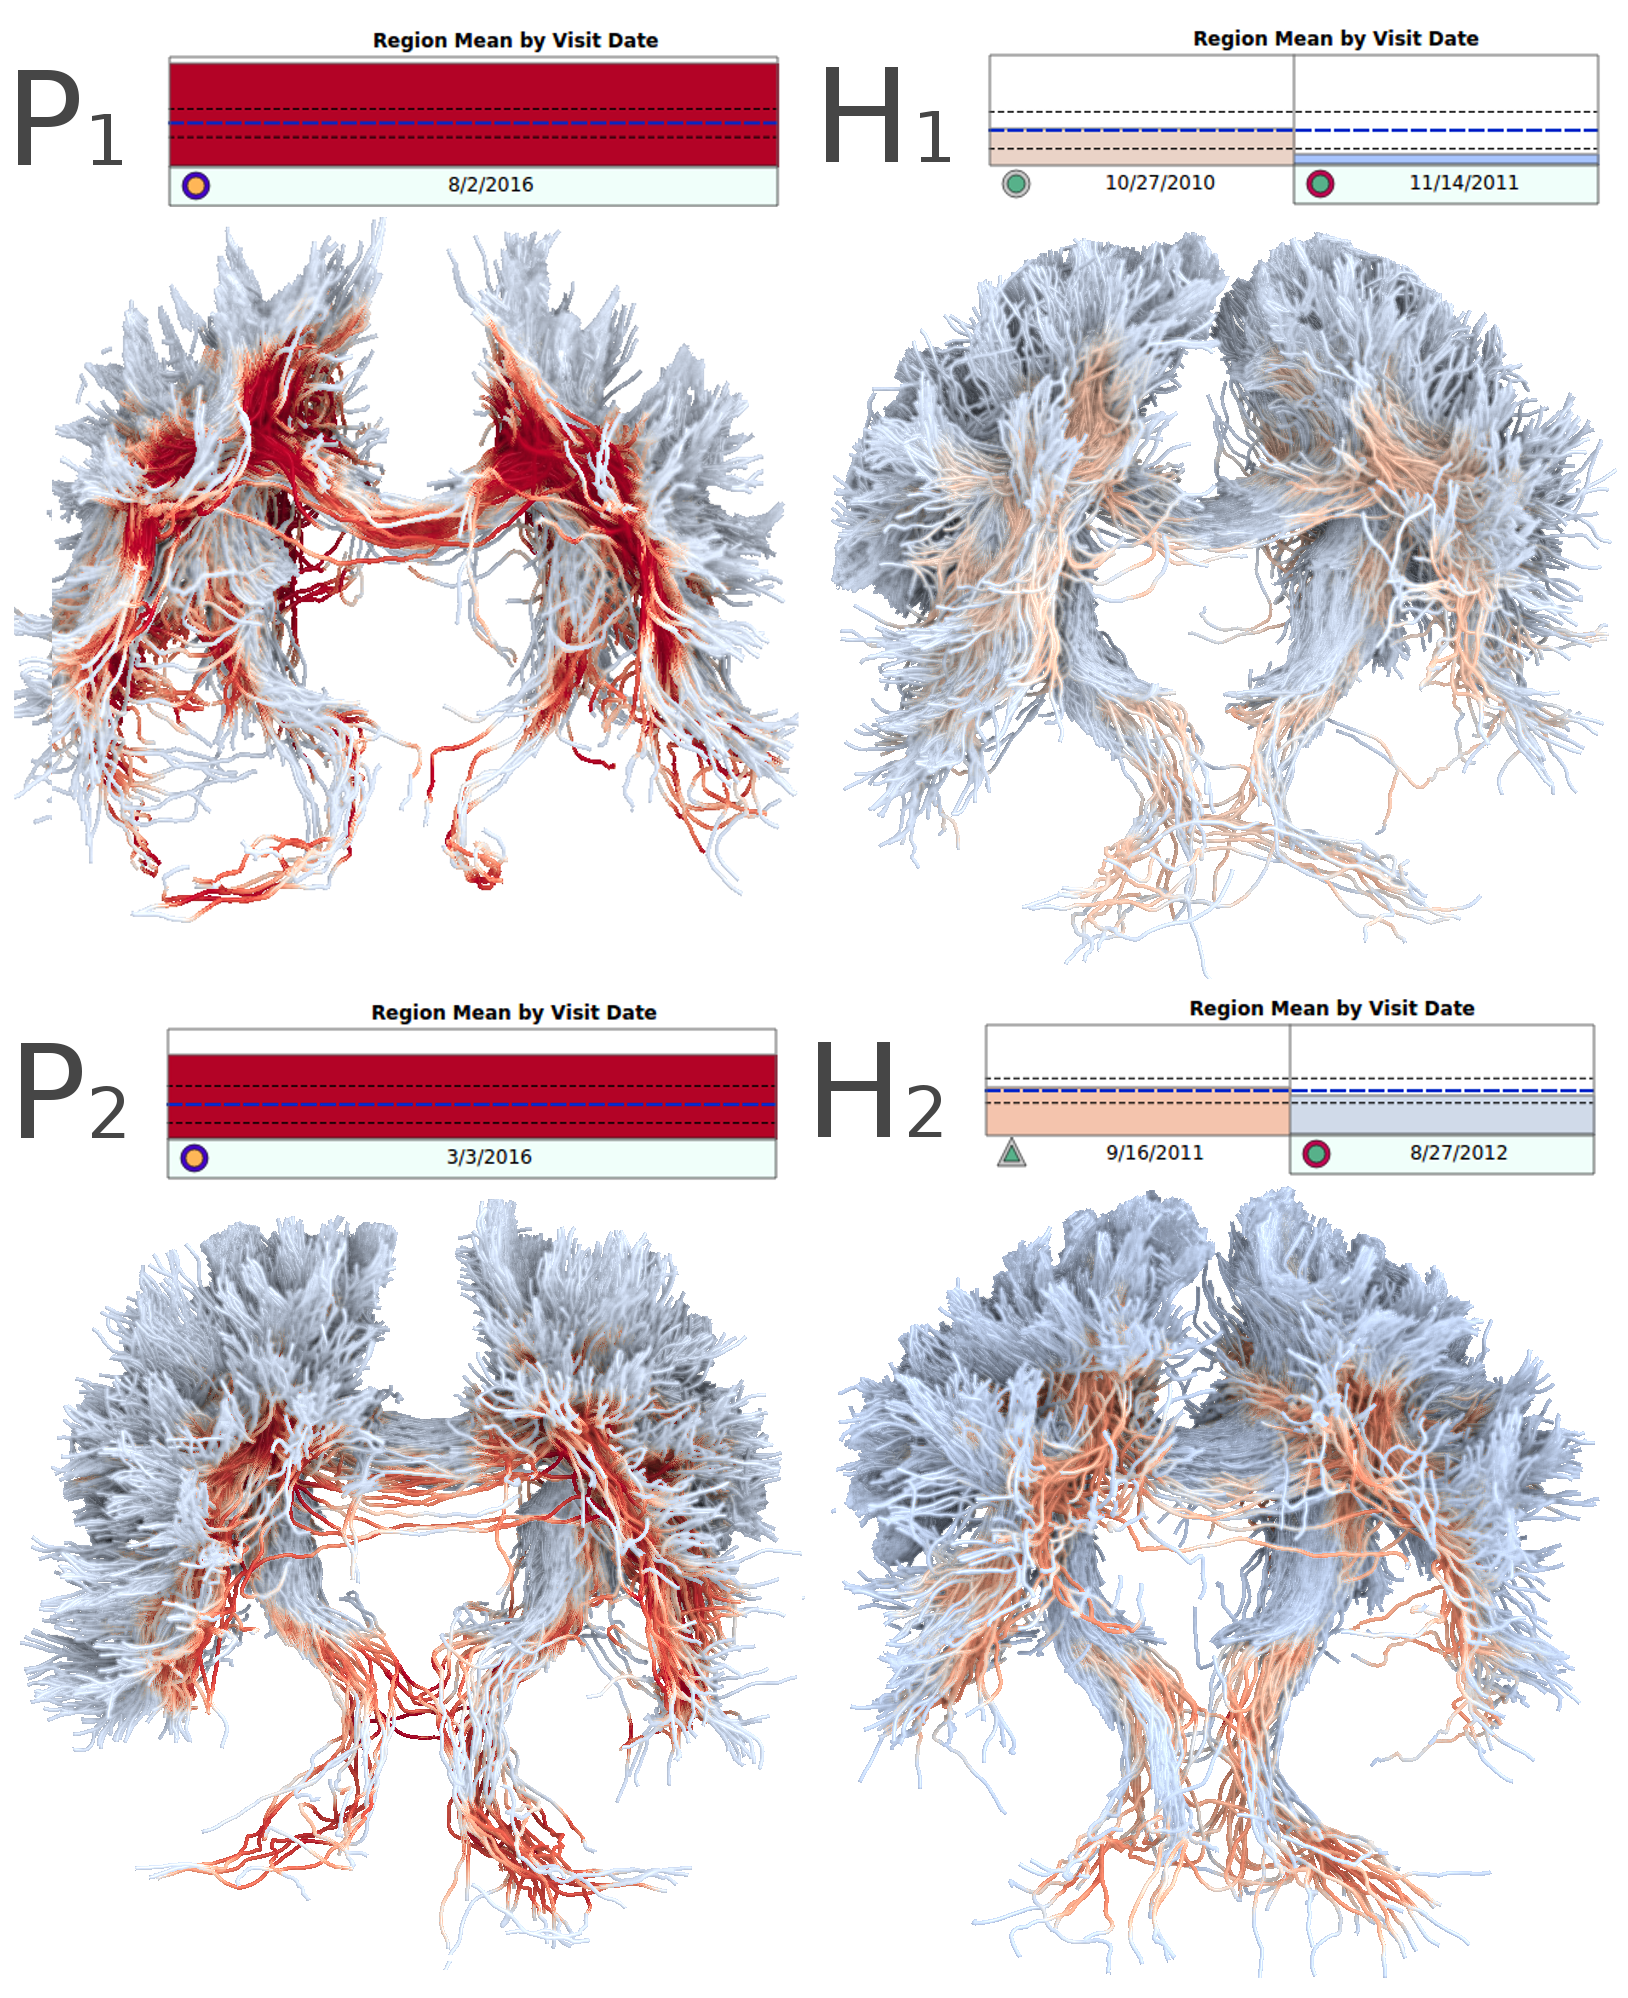
\includegraphics[width=0.9\textwidth]{pregion.png}
% \caption{Some examples mapping the Raw T2 signal with no diffusion weighting (S0) to the Post Central Region. On the left column we show two subjects from the disease group with a noticeable trend that we found to be mildly more prevalent in the disease group. On the right side we show two control group subjects for comparison.}
% \label{fig:pregion}
% \end{figure}

% \subsection{Case Study 2: Effects of Parkinson's on the Postcentral Region }

% In this case study, we gained an overview of the data and analyzed the data set without prior hypothesis. Based on the ML prediction results, we make new hypothesis that Postcentral region might has a strong influence on PD and investigated it through comparative visual analysis, which incorporating both information visualization and 3D rendering of the fiber tracts. 

% According to our system's forecast results, one of the top ranked region for prediction was the Postcentral region and the highest ranked feature within the region was the raw T2 signal with no diffusion weighting (S0). Based on those findings, we assume that the S0 feature in Postcentral region would have high probability of distinguishing between disease and non-disease. The distribution of the feature and scatter plot of all the subjects are shown in Fig.~\ref{fig:PMSO}. From the distribution view of the feature the mean value of S0 in PD is higher than the mean value of control group. In addition, the scatter plot shows the degree of discrimination between the two groups by using this feature. In order to explore the details in spatial space, the fiber tracts that passed through Postcentral region have been rendered in 3D space and the corresponding S0 features have been mapped to the fiber tracts based on their values. We investigated the feature values on the fibers in the physical space and found a trend similar to the trend we found for this feature in the SN region. Several images of the fiber rendering for this case are shown in Fig.~\ref{fig:pregion}. From the fiber rendering view, the fiber tracts of subjects are rendered deeper than those fiber of health. Similarly, from the timeline view, the mean values of S0 in disease subjects are much higher than the mean values of control group. Overall, it seems that the PD shows more subjects with higher values in the inner section of the region. 

% Though more detection about the disease on Postcentral region and S0 feature should be carried out and we are not able to verify how Postcentral region and S0 feature biologically affect PD, our system allows the researchers to have an overview of all the data and provides them with more hypothesis for further study. 



% \begin{figure*}[ht]
% \centering
% \includegraphics[width=1.0\textwidth]{images/fusiformCase.png}
% \caption{ Some examples mapping mean mode of the anisotropy (MMO) to the Fusiform Region. \circled{\small{a} and \circled{\small{b}} } show 3 subjects in different time steps from the PD group and HC group, with a noticeable trend that we found to be more red fiber tracts in the disease group, especially those fiber tracts on Inferior-Superior direction. \circled{\small{c} and \circled{\small{d}} } show MMO feature mapping to the whole brain fibers. There's a noticeable trend that the disease group subjects contain much more dark red spots and blue spots on the brain surface than those in control group.}
% \label{fig:fusiformCase}
% \end{figure*}


% \begin{figure*}[t]
% \centering
% 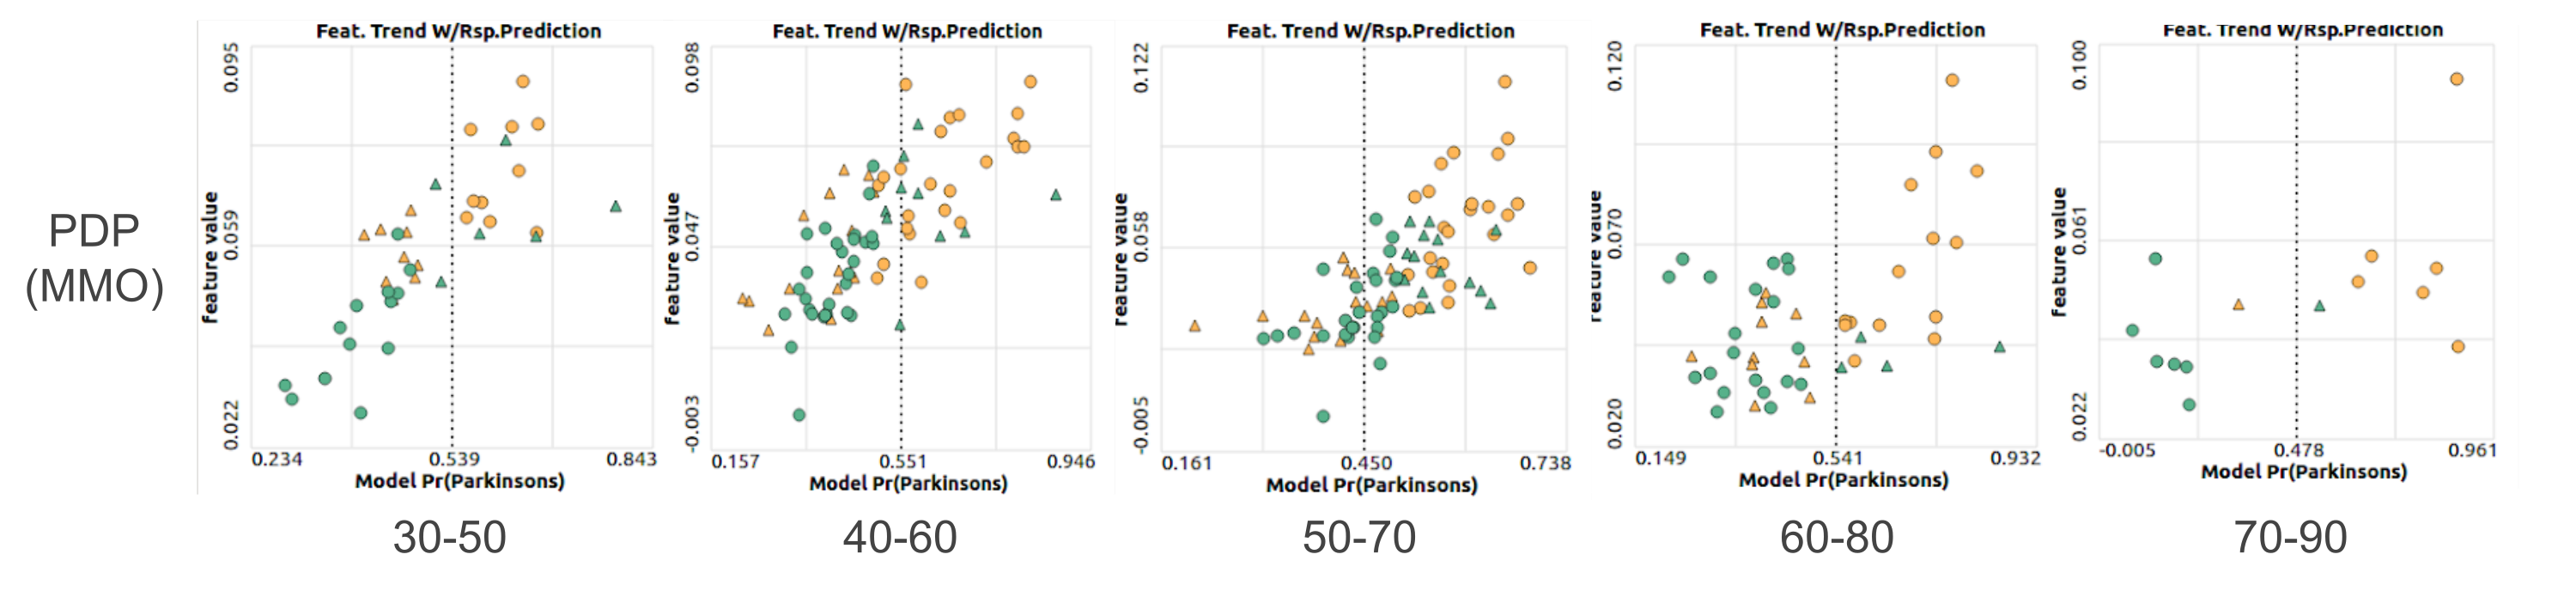
\includegraphics[width=0.85\textwidth]{images/PDP_MMO.png}
% \caption{Partial dependence plots of MMO feature in different ages. It shows strong correlation with PD in young ages}
% \label{fig:FG_PDP_MO}
% \end{figure*}


% \begin{figure}[t]
% \centering
% 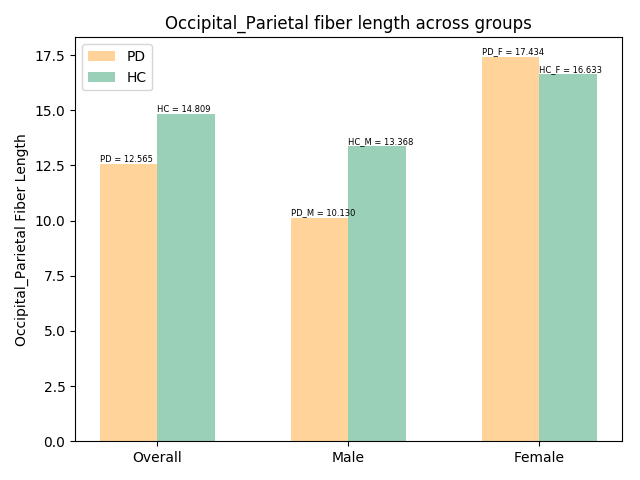
\includegraphics[width=0.95\textwidth]{images/Occipital_Parietal_Groups.png}
% \caption{ Average length of fibers connecting Occipital lobe and Parietal lobe. Overall, the fibers in HC group are longer than those in PD group, while female fiber length are longer than male's.}
% \label{fig:Occipital_Parietal_Groups}
% \end{figure}

% \begin{figure}[t]
% \centering
% 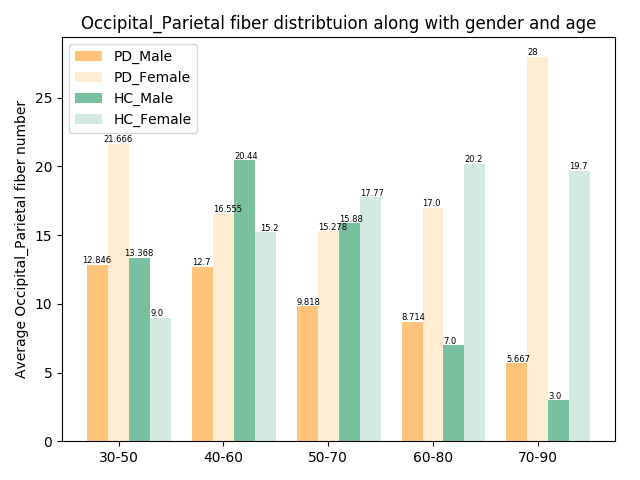
\includegraphics[width=0.95\textwidth]{images/Occipital_Parietal_gender_ages.png}
% \caption{ Average length of fibers connecting Occipital lobe and Parietal lobe. Overall, the fibers in HC group are longer than those in PD group, while female fiber length are longer than male's.}
% \label{fig:Occipital_Parietal_gender_ages}
% \end{figure}


% \begin{figure}[t]
% \centering
% 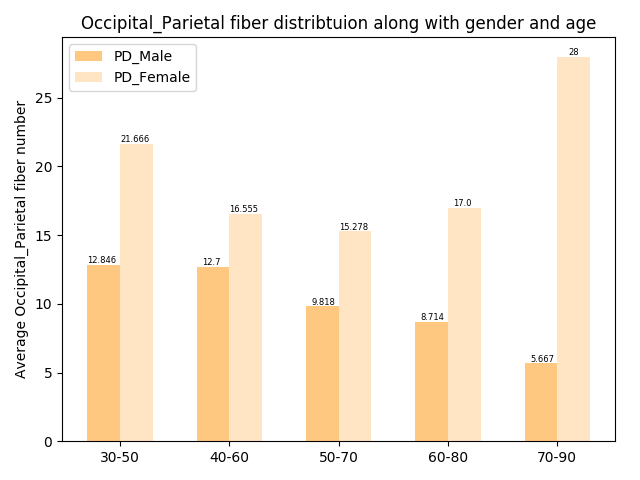
\includegraphics[width=0.95\textwidth]{images/Occipital_Parietal_gender_ages_PD.png}
% \caption{s.}
% \label{fig:Occipital_Parietal_AGE_PD}
% \end{figure}


% \begin{figure}[t]
% \centering
% 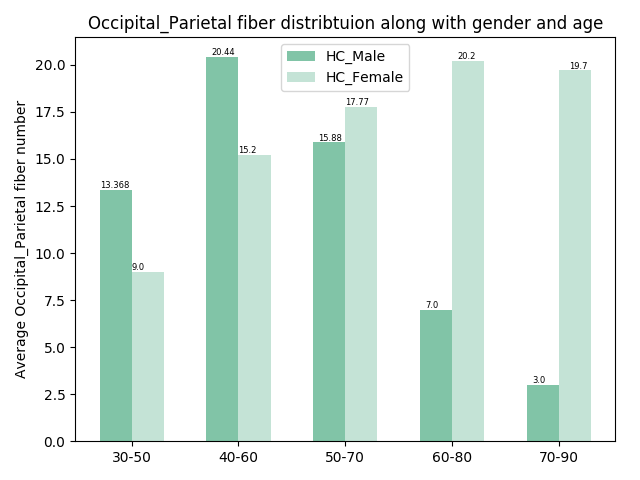
\includegraphics[width=0.95\textwidth]{images/Occipital_Parietal_gender_ages_HC.png}
% \caption{s.}
% \label{fig:Occipital_Parietal_AGE_HC}
% \end{figure}

% \subsection{Case Study 2: Exploration of Parkinson's Disease and the Fusiform Region}% (a hypothesis generation analysis)}

\subsection{Study 2: Exploration of PD with the Fusiform ROI}

% Additionally, we explored the fiber structure difference between HC and PD groups. Besides, age/gender-based exploration has been provided. Based on these analyses, we then provide new hypothesis which potentially would help in early oneset disease detection. 

\noindent In this study, we use our system with no assumptions to explore based on the estimated saliencies. We were interested in the following tasks: explore the brain regions that our system estimates to be the best predictors of PD, %based on our data, 
explore the top performing features in those salient regions, explore patterns of those features dis-aggregated and rendered in the physical space, and explore trends with age and gender.  

% We began by re-sampling our entire dataset without age restriction, and with stratification to balance our cohorts in class, age and gender (Fig.~\ref{fig:fusformSteps} \glf{A}). In total, we obtained 137 subjects, including 68 Parkinson's subjects and 69 healthy subjects. The demographics are shown in (\textbf{\textit{a2}}).

% While clicking the feature of interest in Fig.~\ref{fig:fusformSteps} \glf{C}, the information visualization views (Fig.~\ref{fig:fusformSteps} \glf{D}) show up without delay. After then, subjects are selected from the subjects performance table view (\textbf{\textit{c2}}) and the corresponding fiber tracts of this region are rendered side by side in the juxta-positioned 3D rendering views (Fig.~\ref{fig:fusformSteps} \glf{E}). 

We began by testing our system with the full set of subjects, including 68 PD subjects and 68 HC subjects. The balances in age and gender are shown in Fig.~\ref{fig:fusformSteps} \textbf{\textit{a2}}. After running the pipeline, our system estimated the fusiform ROI to be the best predictor by a small margin (Fig.\ref{fig:fusformSteps} \textbf{\textit{c1}}). The prediction accuracy is 70.1\% and $F_1$ is 0.701. The ROC curve helps show the variability of the classification performance, which gives insight into the uncertainty in the estimated region saliencies and subject prediction scores (Fig.~\ref{fig:fusformSteps} \glf{B}). The top performing feature within fusiform was mode of anisotropy (MO), which is a shape metric representing diffusion patterns (\textbf{\textit{c2}}). We noted that MO was also a top performing feature for many other regions, as well as the whole brain put together. The importance scrores for the 3 modalities of exploration are displayed in Fig.~\ref{fig:fusformSteps} \glf{C}. After selecting the fusiform region (\textbf{\textit{c1}}), we then select MO (\textbf{\textit{c2}}) and begin group and subject (\textbf{\textit{c3}}) level analysis. 

Group level analysis is done using several information visualization views. The parallel coordinates view (\textbf{\textit{d1}}) shows the trends of the top $K$ features. We can see that there is a high variation between subjects, and a lot of overlap in the distributions, while MO clearly shows the most notable differences. Plotting MO vs Pr(PD) (\textbf{\textit{d2}}) helps gain insight into the relationship between mean MO (MMO) to the classification model. An upward trend is noted, while the spread along the vertical axis suggests that other features are significantly taken into account for classification (motivating multivariate analysis). The covariance matrix view \textbf{\textit{d3}} is used to reveal relationships among the different features, and how those relationships differ between the groups. Fig.~\ref{fig:infovis} shows 2 example insights, while Fig.~\ref{fig:fusformSteps} \textbf{\textit{d3}} shows an additional example, where we see high covariance between f-SMS0 and f-MS0 (raw T2 signals in inter-connected and intra-connected fibers respectively). A basic group level comparison of MO is shown in the histogram view (Fig.~\ref{fig:infovis} \glf{D}). Additional comparisons with the fusiform region are shown in Fig.~\ref{fig:infovis}. 

After selecting two interesting subjects, the fibers are rendered in the 3D views and colored by MO. As we have found that the PD group has higher overall mean MO values, we inspect the dis-aggregated MO values as they are distributed on the fibers to look for patterns. For some HC subjects with low mean MO, we find a tendency to have a fuller set of fibers around the lower, outer egdes as can be seen in Fig.~\ref{fig:fusformSteps} \glf{E} and in another example Fig.~\ref{fig:infovis} \glf{E}. Those areas tend to also have lower MO values for both groups. Another common structural characteristic is that some subjects have fewer fibers connecting the occipital and parietal lobes; the ellipse parts in Fig.~\ref{fig:fusformSteps} \glf{E}. This is an interesting to feature to investigate further, since reduced fiber density connecting between the occipital and parietal lobes has been suggested to be a possible sign of diseased brain atrophy in PD~\cite{10.1093/brain/awh088}. 

Besides focusing on the fusiform, we also toggle between the whole brain colored by MO (Fig.~\ref{fig:fusformSteps} \glf{F}). While we notice higher values tend to be in the same areas for both groups, we notice some anomalies as shown in Fig.~\ref{fig:fusformSteps} \glf{E}, \glf{F}, where we discover large patches of high values (red) in a selected PD subject with high mean MO. These non-uniform higher intensity regions may be a factor in the predictive model, and we notice they tend to be found more in certain areas than others, which could inspire a further effort to localize and understand the cause. In the physiological sense, the different distributions of MO intensity indicate different patterns of water diffuse in different parts of the brain; however, imaging issues could also affect these tensor measures.

The insights we found, based on exploring in the physical space, is that it's not simply the case that the PD group has higher MO values, but rather that they may also have a different overall balance of fiber density in specific areas; those structural differences impact the average values since different areas tend to have higher or lower values in any case. This highlights that the impact of the tensor measure distributions in physical space is an important factor to consider (in relation to the average use for ML), and this factor is linked to structural differences between subjects as well. Since each brain is unique, both in relative local fiber density and in MO distribution, analysis of the feature can benefit greatly from inspecting in the physical space where these details can be observed, stressing the value of linked 3D visualization.  

In Fig.~\ref{fig:fusformSteps} \glf{G}, trends with age alone (\textbf{\textit{G1}}), and additionally with gender (\textbf{\textit{G2}}) are explored. Overall, the PD subjects have higher MO. However, as shown in \textbf{\textit{H2}}, the trend for the male and female subjects shows different patterns; on average, for the male subjects, MO decreased in age, while for females MO increased with age. However, the limited amount of data (especially in elderly female PD subjects) makes this insight highly uncertain; further investigation would be necessary. 


% In addition, with selecting different time steps of a subject in the timeline views, we can have visual sense of the disease progress. Integrating brain region rendering, whole brain rendering and the subjects in different time steps, user would have a qualitative understanding of PD effects in physical space. Through empirical analysis, we discover more red spots and blue spots on the surface of the whole brain in the PD group than those in the HC group, especially in those subjects predicted true positive (TP) and true negative (TN). \textbf{(Task 1)}.  

% Back to the brain feature table view (\textbf{\textit{c3}}), the mean mode of the anisotropy ( MMO ) is a salient feature that is listed on the top of the table with low standard deviation. With clicking this feature, information visualization views of this feature would be shown in Fig.~\ref{fig:fusformSteps} \glf{D}. 

% Moreover, inspired by the performance of MMO in \textbf{\textit{d2}} and Fig.~\ref{fig:fusformSteps}  \glf{I}, we show our interest in the MMO feature effects at different ages. Splitting the dataset into $5$ subgroups as shown in Fig.~\ref{fig:groupDemographics}, we executed the ML pipeline multiple times with each subgroup subjects and obtained several partial dependence plots of MMO features at different ages (Fig.~\ref{fig:FG_PDP_MO}). Each subplot shows the relation between MMO feature and prediction outcome. The correlation between MMO and disease prediction is gradually weakening with age growth. In contrast to AFL of nigrostriatal fibers effects on PD in the previous case, it implies the MMO feature has a greater impact on the early PD. Since then, we may provide a hypothesis that MMO feature of one's brain might be relevant to the pathological characters of PD. Furthermore, it may potentially contribute to form a marker to identify early PD \textbf{(Task 3)}. 


% \subsubsection{Analysis and Insights}

% During the exploration process, we observe the disparity of fiber connection and the spots distribution difference between the HC group and the PD group. 


% The differences in MO intensity as they appear distributed on the fibers, indicates different patterns of how water molecules diffuse in different parts of the brain. We find it interesting, especially how the fiber structure, and relative density of fibers throughout the region can strongly have an impact on how the average, since there is also a strong correlation between region and MO intensity. 

% % More red spots and blue spots in PD brains may indicate a higher degree of water diffusion freedom. 

% Further analysis of such patterns may help neuroscients better understand how the disease spread in one's brain. Since these two manifestations appear to be more frequent incorrectly classified subjects than them in false predicted subjects, we suspect them contribute a lot to the model predictions.   

% According to the line charts of the MMO feature with respect to ages and genders, we find that PD is highly related to these two factors. \textbf{\textit{I1}} reveals that both the two groups have decline trends, but the value of MMO tends to be relatively higher in the PD group than it in the HC group. Moreover, with advancing age the MMO value overall has a decreasing tendency. This pattern could also be found in the male group in \textbf{\textit{I2}} (the solid lines). oppositely, the female group in \textbf{\textit{I2}} (the dotted lines) shows a relatively different pattern that have a promotion trend in elder ages. However, it may be biases that caused by the limited female subjects in the two groups, especially in the elder ages, as seen in Fig.~\ref{fig:groupDemographics}. Based on these findings, we could assume that the tendency in \textbf{\textit{I1}} is in a large part caused by males in \textbf{\textit{I2}}. Furthermore, we could make an assumption that men may be more likely to develop PD than women, which has been validated by researchers.\cite{Haaxma819}

 

 
%displays MMO value changes with advancing age and the MMO patterns on genders. We can clearly see different patterns in male and female groups, where male group shows decline trends with ages, but the female group seems to have a promotion trend in elder ages. However, it may be biases that caused by the limited female subjects in the two groups, especially in the elder ages, as seen in Fig.~\ref{fig:groupDemographics}

%For example, regarding the \textit{Air Force One } and \textit{Jumps} video (as shown in \autoref{case2_4}), the value of \textit{motion} score tends to be relatively higher, while the \textit{memory} and \textit{aesthetics} tend to be lower. This pattern could also be found in a bunch of videos of different types.
%However, the impact of such pattern varies among different video types, 




% Though many other fiber-tract based features like fiber number/ fiber length can differentiate PD group from HC, group , the current visual representation method, which just average the features and map them to fiber tracts, is still not good enough to show such features. The other tensor based features also show the capability to distinguish those two groups, it may not be obvious to see the features change when mapping them to the fiber tracts. MO feature in Fusiform region shows the changes both in physical structure as well as features distribution

% First, the fiber tracts go through the fusiform region. ( we call it single region fiber tracts ). Fig.~\ref{fig:fusiformCase} shows the fibers in PD group has more red fibers, which represent higher MO values have been mapped to the fiber tracts, than those in HC group. Even more, more fiber tracts on Inferior-Superior (I-S) direction, connecting from fusiform brain region and frontal lobe, especially caudal middle frontal and rostral middle frontal, have been found in PD group than those in HC group.   

% Second, from the whole brain fiber tracts, seen in Fig.~\ref{fig:fusformSteps} we can see much more and dark red spots or blue spots on the surface of the PD brains than in HC group brains. The brains with an extremely large amount of red surface are all in the TP group and FP group, where the healthy brains are predicted to be a diseased brain. While none brain that is characterized by an extremely large amount of red surface has been found in TN group and only one brain with such a trait in TN group has been FN group, where the disease brains are predicted to be a healthy brain.

% After exploring the data with our system, we can make a hypothesis that  the fiber tracts with darker red colors mapped to them on the brain surface in PD group might be affected by those red fibers connecting fusiform brain region and frontal lobe, where we can see the fiber tracts inside the dotted circle in Fig.~\ref{fig:fusformSteps}(E). Moreover, we make a hypothesis that those fibers might have a strong relationship with the disease. 

% Furthermore, we investigate which subjects contribute most to disease prediction and counting how much contribution to the predictions. Because we were using 5 folds cross-validation, we select the top N subjects, ranging from 6 to 30, from TP and TN groups. After running the ML pipeline multiple times, we got the accuracies of the top N subjects. From the accuracy curve in Fig.~\ref{fig:TopNaccPlot}, we observed that the classification accuracy goes to more than 85\% with top 16 subjects in each group, which implies those subjects contribute a lot to the predictions while using all the subjects in all ages. 

% To test those hypothesis, we perform a statistical analysis out of our system. we took all these brain fibers, from single region or whole brain, screenshots down and divided those screenshots into 4 groups, which are based on the prediction results ( TP, TN ,FP ,FN ) , respectively. Totally, we have 18 subjects in FP group, the minimum number of the 4 groups. We regard the top 18 brain with the highest prediction probability can be used to represent TN/TP group to a large extent. Here we consider top 18 brains in TP and TN groups, and top 18 brains in FP and FN groups. (Totally,  our dataset contains 68 HC subjects, in which 50 subjects in TN group and 18 subjects in FP group,  and 69 PD subjects, in which 45 subjects are in TP group and 24 subjects are in FN group ) 

% To test the first hypothesis, We perform a qualitative comparison, which is based on the red and blue spot coverage of the brain surface, in the 4 groups of the whole brain fibers. Fig.~\ref{fig:Fusiform_Spotcoverage} indicate the 

% We classify brains into 5 levels in visual perception. The more red on the brain surface, the lower the level is. Fig 20 shows the distributions of each group. It is easy to find the TP and FP groups have similar distributions, while the TN and FN groups have other distributions.

% In the 4 groups of the single region fibers, qualitative observation of the number of I-S fibers has been carried out. If the brain contains few fiber tracts, we mark it ``1'', conversely, we mark the brain as ``0''.  Then we come to the result, which is shown in Fig 21, that the HC and FN groups had a higher fiber reduction rate(  the ratio of ``1'' in the group ) than it in PD and FP groups. 

% Thence, our system supports  new  hypothesis generation  and  hypothesis-driven  analysis  of  the  disease. Moreover, our system can, to some extent, explain why the brain is predicted to be disease/healthy.

% \begin{figure}[t]
% \centering
% 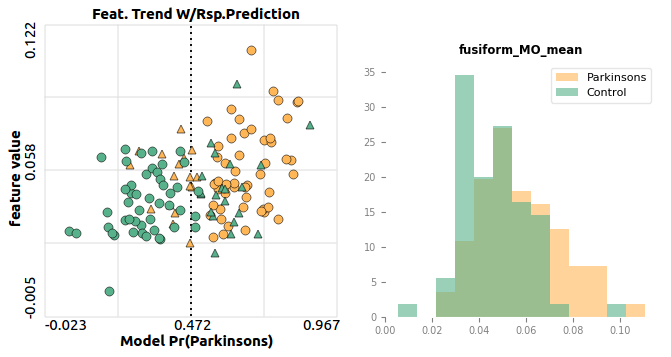
\includegraphics[width=0.9\textwidth]{images/Fusiform_MMO_distribution.png}
% \caption{Comparing the distributions of the MMO feature ( mean mode of the anisotropy ) between the control group (blue-green) and disease group (orange). The disease group’s distribution is centering at a higher value than the control group and there are few outliers from the health group in the high value range.}
% \label{fig:fusform_distribution}
% \end{figure}


% \begin{figure}[t]
% \centering
% 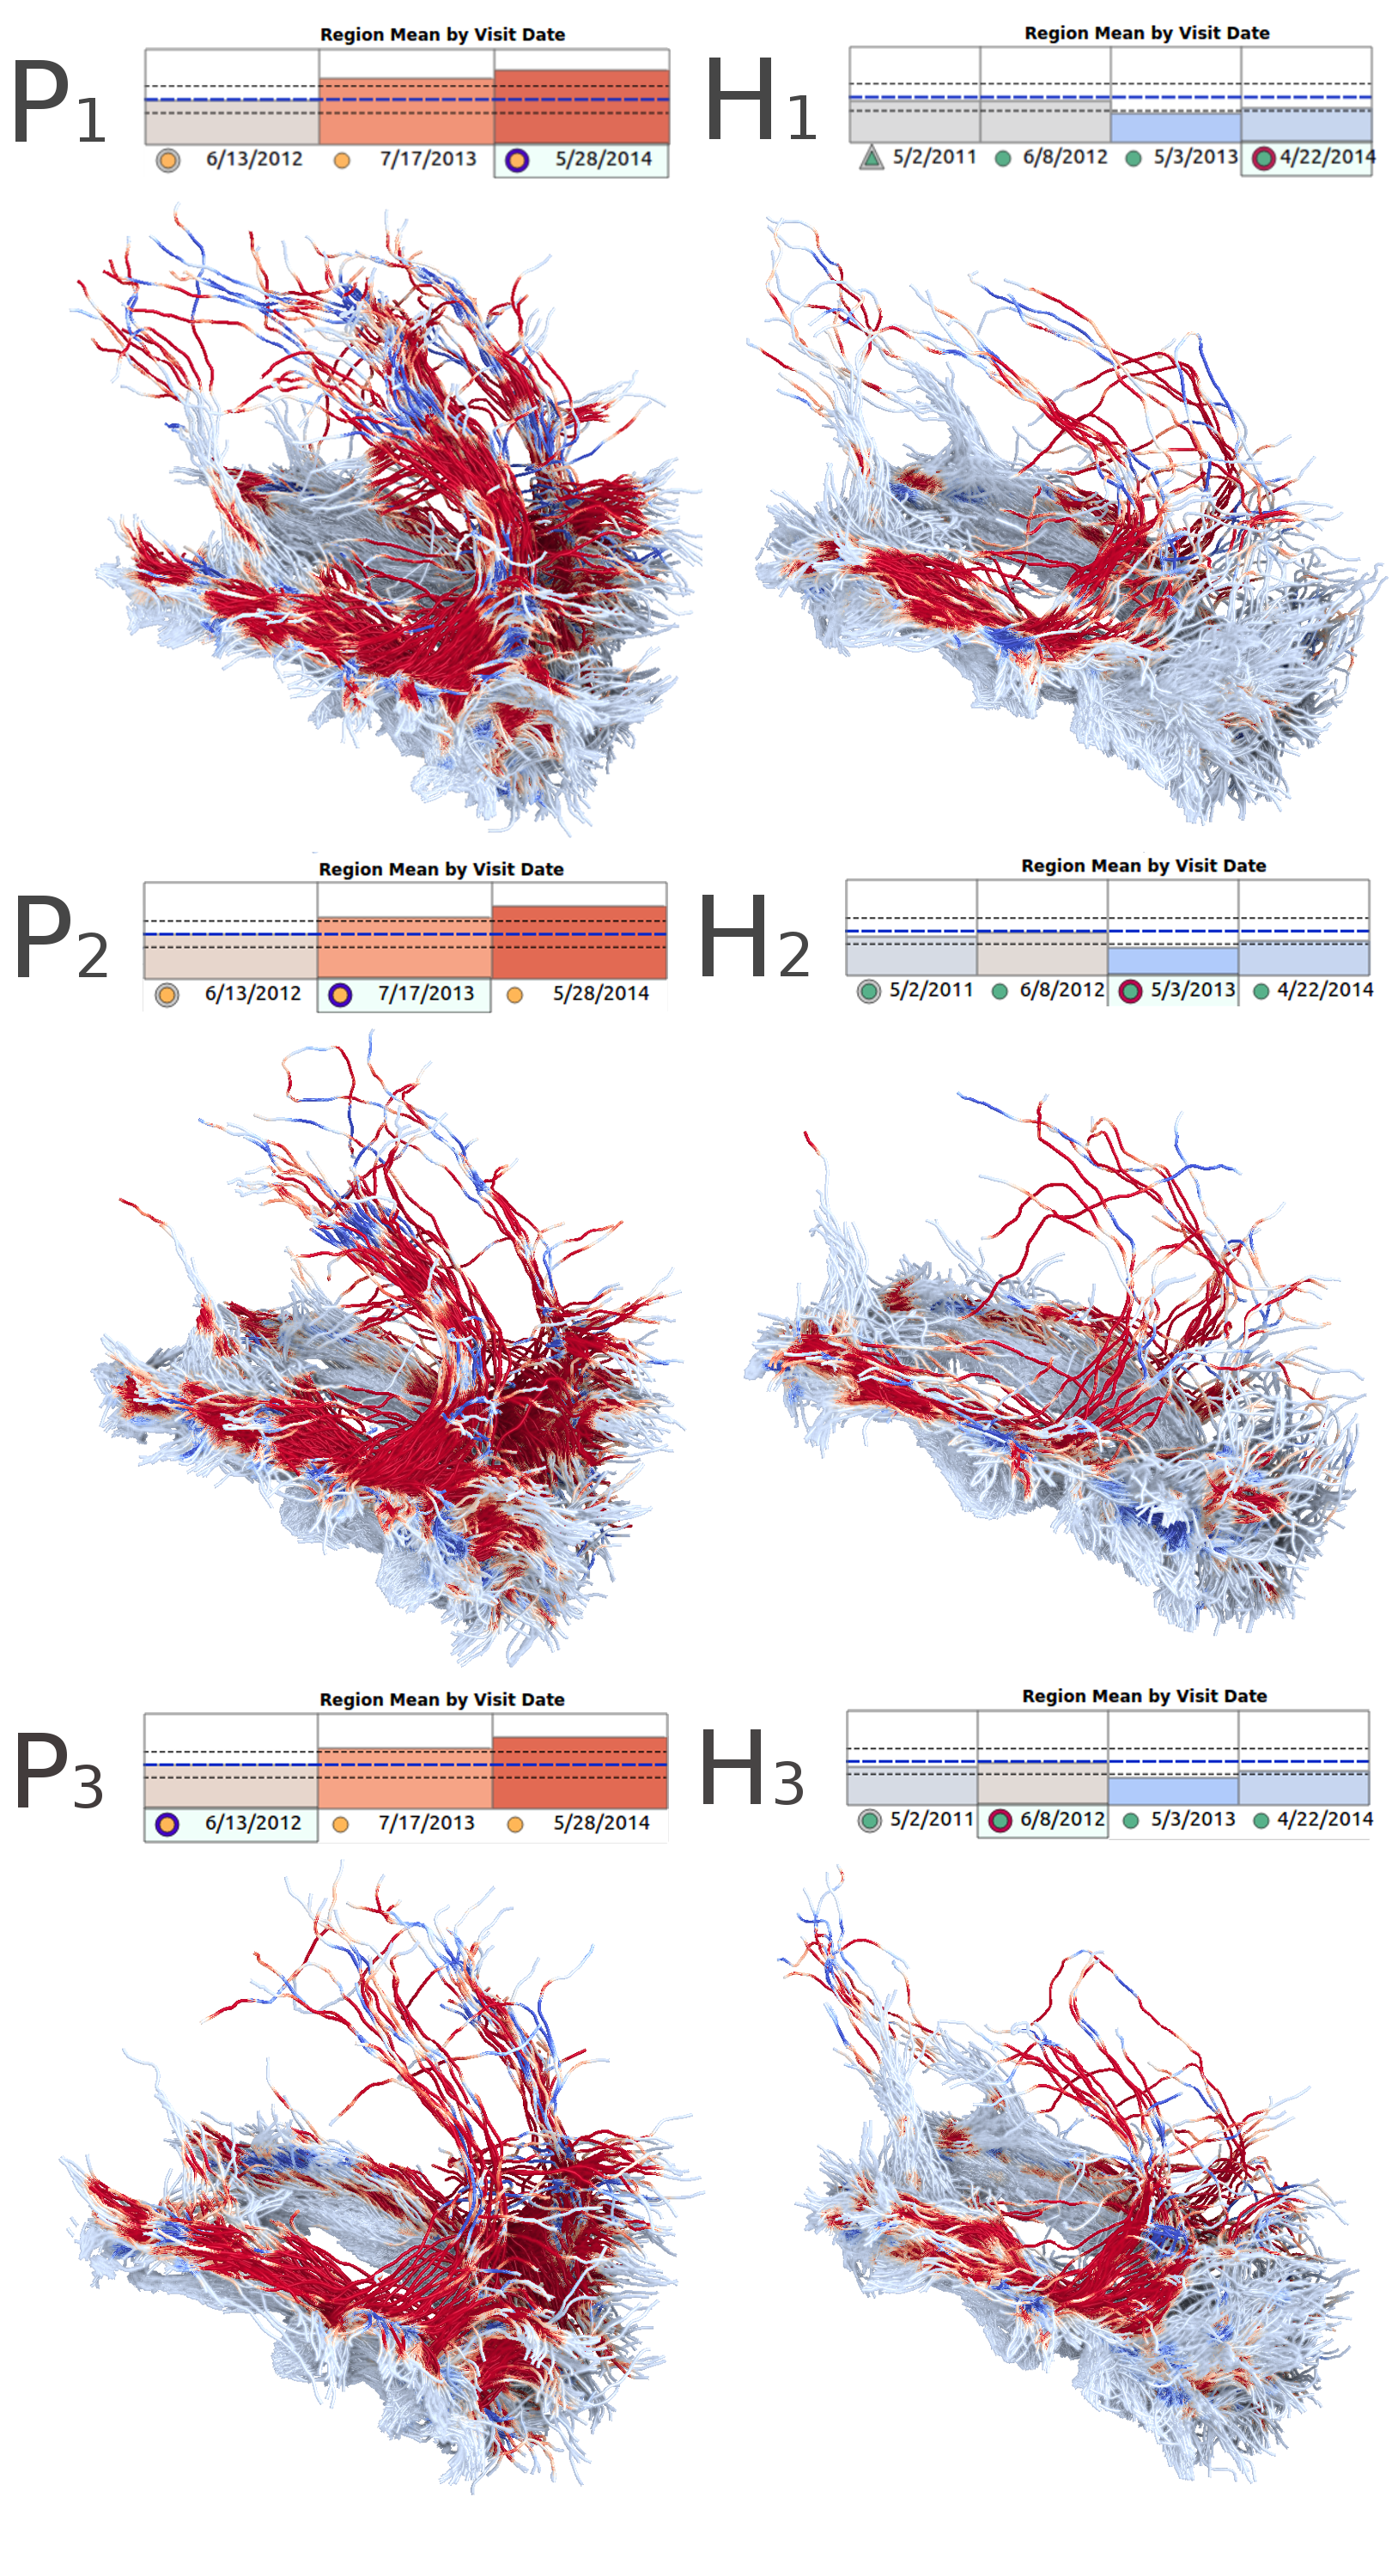
\includegraphics[width=1.0\textwidth]{images/Fusiform_MMO_Region.png}
% \caption{Some examples mapping mean mode of the anisotropy (MMO) to the Fusiform Region. On the left column we show 3 subjects in different time steps from the PD group with a noticeable trend that we found to be more red fiber tracts in the disease group, especially those fiber tracts on I-S direction. On the right side we show 3 control group subjects in different time steps for comparison. }
% \label{fig:fusform_region}
% \end{figure}

% \begin{figure}[!ht]
% \centering
% \includegraphics[width=1.0\textwidth]{images/fusiform_MMO.png}
% \caption{Some examples mapping the MMO feature to the whole brain fibers. The subjects are the same as that of the Fig.~\ref{fig:fusform_region}. There's a noticeable trend that the disease group subjects contain much more dark red spots or blue spots on the surface than those in control group. }
% \label{fig:fusform_surface}
% \end{figure}

% \begin{figure}[!ht]
% \centering
% 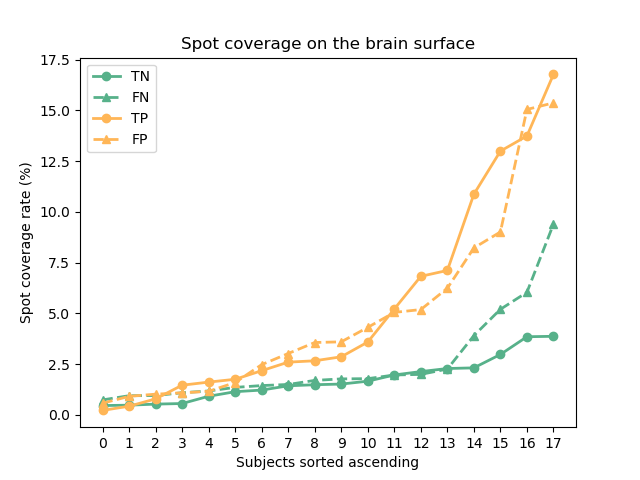
\includegraphics[width=0.9\textwidth]{images/Fusiform_Spotcoverage.png}
% \caption{.}
% \label{fig:Fusiform_Spotcoverage}
% \end{figure}
% \begin{figure}[!ht]
% \centering
% 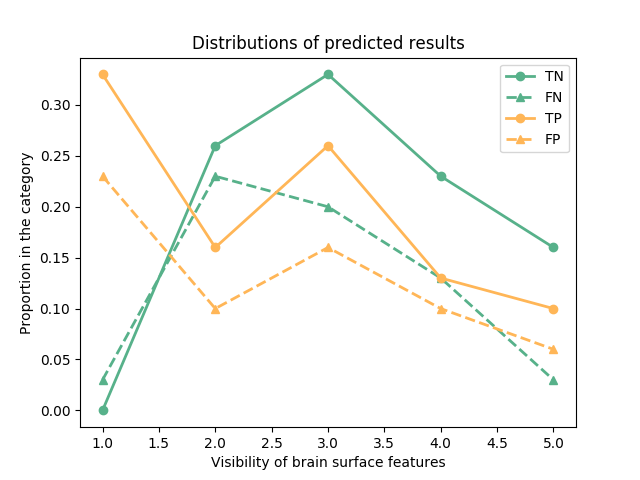
\includegraphics[width=0.9\textwidth]{images/Fusiform_BrainimageDistribution.png}
% \caption{.}
% \label{fig:Fusiform_BrainimageDistribution}
% \end{figure}

% \begin{figure}[!ht]
% \centering
% 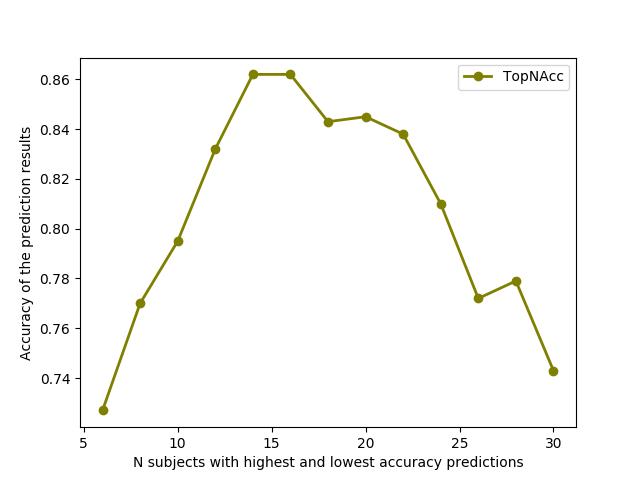
\includegraphics[width=0.9\textwidth]{images/TopNaccPlot.png}
% \caption{ Top $n$ subjects prediction accuracy. Selecting $n$ subjects from TP and TN groups, the prediction accuracy first increase then decrease with $n$ increase.}
% \label{fig:TopNaccPlot}
% \end{figure}

%\begin{figure}[!ht]
%\centering
%\includegraphics[width=0.9\textwidth]{images/fusiform_MO_distribution_wholebrain.png}
%\caption{we don't need it, just show how we get the figure 20}
%\label{fig:fusform_Mo_distribution_wholebrain}
%\end{figure}

%\begin{figure}[!ht]
%\centering
%\includegraphics[width=0.9\textwidth]{images/fusiform_MO_distribution_singleregion.png}
%\caption{we don't need it, just show how we get the figure 21}
%\label{fig:fusform_Mo_distribution_wholebrain_singleregion}
%\end{figure}

%On top of the fiber rendering view is the subjects information and their timeline showing their mean values of the selected feature against the control group mean for each of the subjects scans.

\vspace*{-0.06in}
\subsection{Expert Feedback}

\noindent Our team includes computer scientists with expertise in machine learning and visual analytics, and a computer scientist with some prior experience studying fiber tracts in an interdisciplinary lab. To help evaluate our work, we sought feedback from 2 domain experts, each with unique perspectives and backgrounds in neuroscience. The first (E1) is a neuroscientist with expertise in statistical analysis, tractography, and neurodenerative disease. The second (E2) is a neurologist at a children's hospital specializing in diagnosis and treatment of congenital nervous system malformations, and voxel-based morphometry (VBM) analysis of Huntington's disease.
%various congenital nervous system malformations, as well as brain trauma, tumors, and Huntington's disease.
%congenital nervous system malformations such as hydrocephalus, arachnoid cyst, tethered spinal chord, brain trauma, brain tumors, and Huntington's disease (a type of neurodenerative disease). 
We conducted live interactive demos to each of them, and also shared a draft of our manuscript. We then assimilated the feedback into our design and paper.

E1's assessment reflects an interest in DTI and fiber based bio-marker research. Since fiber based analysis of neurodenerative disease is still in the early stages, E1 said current research is highly exploratory. Advanced methods such as fiber tractography are emerging with promise for scientific discovery, however the complexity and uncertainty present daunting challenges which can be intimidating and "scare some researchers" away E1 said. In E1's experience: due to those complexities, limitations in their arsenal of software, and practical difficulty comparing many different individuals in the physical space; the focus tends to be more on statistical comparisons (e.g. DTI measures averaged in ROIs) than analysis of individual fiber tracts directly. For E1, physical analysis is usually initiated to investigate outliers. Overall, E1 thought that the system could make it more practical to do a deeper physical analysis than they normally. To E1, the concept of using AI to guide an exploratory VA process was new. E1 expressed concern that many neuroscientists don't have a background in ML, and that difficulty understanding ML models, parameters, and inputs, could be a discouraging factor. Since this is a novel area of research, the full impact that it will have is not completely understood.

E2 thought the tool was innovative and useful as a research tool, but as a medical doctor was interested to envision how the work could eventually impact clinical practice. For research, the doctor said it could help in studying neurological disease from a new perspective. The expert believed that better understanding of changes in the fiber tracts could offer a new perspective into the morphological aspects of brain disease. However, in clinical practice, E2 expressed that only well understood and standardized markers can be translated into actionable insight. E2 also suggested that for clinical use a simplified system that hides the AI pipeline would be more usable, and that AI experts may need to be assigned to hospitals for them to properly utilize the technology. The doctor said that currently there are certain bio-markers that are very important in clinical practice for diagnosis and disease evaluation. It was suggested that a promising next step may be to analyze the co-occurrences of those markers with tract based features; in the long run, E2 suggested, those new features can be added as additional index variables in multi-modal disease severity grading systems. This could improve clinical practice by better defining and diagnosing disease characteristics, severity, and progression. While our system is designed for exploratory research, and the current scope is restricted to tract based analysis, we find these comments interesting and useful for VA researchers to plan future work. 
% Still, we note that our current system is able to incorporate other bio-markers into the ML pipeline and VA system so long as the data is available for each subject and can be input into the ML classification model. Besides enhancing prediction performance, and offering additional context and multi-modal insight, if the extra features also have a spatial component, they could be easily linked with the fiber tract ROIs. Still, there will be much room for future work specifically focusing on VA of multi-modal clinical characteristics. 
% As fiber-tract based research into neurodenerative disease matures, and findings are robustly validated, it may provide exciting and impact-full advancements with real world clinical applicability.

\subsection{Performance}
\label{sec:performance}
\noindent As mentioned in Sec.~\ref{sec:aggregation}, the user must wait for the machine learning pipeline to complete before the exploratory analysis. The time that this takes is highly dependent on data size and parameters in the ML pipeline. The most time intensive part of the pipeline comes from the extremely random trees/ensemble based feature importance algorithm that we use by default for feature saliency estimation. This comes with an option to choose the number of trees/estimators, which is linearly correlated with the run time; 150 is the default, but can go as high as 1500 to achieve moderately better results. CV parameters $k$ and $c$ are also linearly correlated with run-time. We tested the performance with a few reasonable settings, over all regions as described in Sec.~\ref{sec:aggregation},  with 136 subjects. The classifier we used was an SVM, and we used the default heuristic to train it on the top $\sqrt{n}$ ranked features (Sec.~\ref{sec:feature-sel}). The test machine had an Intel(R) Core(TM) i3-9100F CPU @ 3.60GHz. With the default parameters (150 estimators/trees, 5 CV folds, and $c=10$ repetitions of CV), the pipeline took 42 seconds. Increasing the number of estimators to 1500, and the CV folds to 10, it took 5 minutes and 25 seconds. These are reasonable wait times, since afterwards the user can explore without hesitation.